\documentclass[a4paper]{book}
\usepackage[T1]{fontenc}%per rappresentare i font italiani, come le lettere accentate, con la giusta spaziatura
\usepackage[utf8]{inputenc}%per poter inserire nel testo .tex i caratteri unicode8
\usepackage[italian]{babel}%per poter effettuare la giusta sillabazione della lingua italiana
\usepackage{classicthesis}%necessario per utilizzare lo stile dell'Ars Classica
\usepackage{arsclassica}% per avere lo stile dell'Arte di imparare il latex
\usepackage{amsmath}%per poter rappresentare ed utilizzare al meglio gli ambienti e le formule matematiche
\usepackage{amssymb}%per rappresentare alcuni simboli particolari matematici
\usepackage{amsthm}%per definire e poter effettuare le dimostrazioni matematiche
%\usepackage{amsfont}%per poter avere i font matematici
\usepackage{booktabs}%per la corretta gestione delle tabelle
\usepackage{graphics}%per effettuare i grafici
\usepackage{pgfplots}%per i grafici
\usepackage{rotating}%per effettuare le rotazioni delle immagini e grafici
\usepackage{microtype}%per effettuare un aggiustamento della spaziatura tra caratteri e del font
\usepackage[cache = false]{minted}
\usepackage{color}
\usepackage{framed}
\usepackage{listings}
\usepackage{url}%per poter rappresentare gli url nel testo latex
%\usepackage{hypertext}%per effettuare un collegamento con una pagina internet
\newtheorem*{defi}{Defi}%Definizione per avere la gestione delle definizioni
\newtheorem*{teorema}{Th}
\newtheorem*{esempio}{Esempio}
\definecolor{shadecolor}{gray}{0.90}

\begin{document}
%Intestazione e indice dei contenuti
\title{Linguaggi di Programmazione}
\author{Marco Natali}
\date{}%rappresenta la data di compilazione del file
\maketitle

\tableofcontents

\chapter{Introduzione ai Paradigmi di Programmazione}
Nel corso di Linguaggi di Programmazione ci occupiamo di 3 importanti paradigmi di
linguaggi quali i linguaggi logici, linguaggi funzionali e linguaggi predicativi, la cui conoscenza è importante
per decidere quale paradigma usare per risolvere un particolare problema e permette di migliorare la
propria competenza nell'ambito della programmazione per scrivere programmi il più possibile efficienti.

Durante il corso, ma soprattutto durante la vita futura lavorativa, si dovrebbero rispettare le regole
standard di rappresentazione e formattazione dei programmi quali ad esempio lo standard Google, regole GNU, per cui nei programmi
sviluppati in questo corso devono rispettare le seguenti convenzioni:
\begin{itemize}
\item ``Usare Emacs come editor in quanto indenta lui al meglio'' cit Antoniotti
\item le linee di codice non devono essere più lunghe di 80 colonne per riga
\item inserire spazi tra gli operatori e uno spazio dopo virgola  e punto e virgola  ossia \textbf{2 + 3} e \textbf{(4, 5)}.
\item non inserire uno spazio tra il nome di una funzione/predicato e le parentesi ossia \textbf{foo(4)}.
\item inserire uno spazio tra un istruzione di controllo/operatori logici e le parentesi ossia \textbf{if (4 || 5)}
\item non usare i commenti all'interno di un box perchè difficilmente mantenibile
\end{itemize}
I linguaggi di programmazione vengono classificati in base a quale paradigma implementano per la computazione, ossia il modello di riferimento
usato per strutturare un programma, al fine di facilitare l'apprendimento di linguaggi similari:
\begin{itemize}
\item \textbf{Imperative Languages}: basati sull'architettura di Von Neumann, utilizzata da tutti i calcolatori moderni,
      in cui il processore ha il compito di leggere e scrivere le celle di memoria durante l'esecuzione della computazione.\newline
      Questo paradigma utilizza uno stile prescrittivo, ossia i programmi iterativi specificano una sequenza
      di istruzioni da eseguire per modificare lo stato del sistema e questo flusso può essere modificato soltanto con
      le strutture di controllo.\newline
      Ne fanno parte il C/C++, i linguaggi Assembler, Pascal, Python, \dots
\item \textbf{Logic Languages}: paradigma in cui un programma è una deduzione logica, ossia ogni istruzione è una formula del linguaggio
  e la computazione consiste nell'interrogare il sistema per sapere se l'interrogazione fa parte della conoscenza rappresentata dal programma.

      Questo paradigma viene utilizzato principalmente per la dimostrazione della correttezza di un programma, per rappresentare i database
      ed infine sta avendo un notevole utilizzo ultimamente nel campo dell'AI(Artificial Intelligence).\newline
      Fa parte di questo paradigma principalmente solo il Prolog e i suoi derivati, infatti noi useremo il SWI-Prolog.
\item \textbf{Functional Languages}: paradigma in cui il concetto di funzione è l'unica cosa importante infatti i programmi
      consistono nell'applicazione e nella definizione di una serie di funzioni.\newline
      Ne fanno parte i linguaggi Lisp, Common Lisp, Scheme, Javascript, ML, Ocaml, Haskell, R e pochi altri.
\end{itemize}
Ognuno dei seguenti paradigmi può essere ad oggetti, come ad esempio Java, C++, Common Lisp, Python,
infatti il paradigma ad oggetti è ortogonale alla definizione data da noi delle diverse tipologie dei linguaggi,
anche se presume alcune caratteristiche tipiche dei linguaggi imperativi.

\section{Paradigma Imperativo}
Il paradigma imperativo, come già visto, si occupa di eseguire una sequenza di istruzioni
infatti fu inventato per la computazione ``numerica'', a differenza degli altri paradigmi che si concentrano sulla computazione simbolica.

Un programma imperativo è composto da due componenti, uno per rappresentare le strutture dati e l'altro per gli algoritmi:
\begin{itemize}
\item dichiarazione in cui vengono dichiarate le variabili, i tipi e le funzioni necessarie per la computazione,
      ossia vengono stabilite le strutture dati necessarie per l'implementazione del programma.
\item definizione in cui si implementatno gli algoritmi, per eseguire correttamente la computazione, utilizzando le istruzioni del linguaggio.
\end{itemize}
Il paradigma imperativo ha spopolato fino agli anni '70/80 quando venne spodestato dal paradigma ad Oggetti e noi lo abbiamo già
affrontato durante il corso Programmazione per cui in sto corso vedremo soltanto alcune peculiarità del linguaggio C,
come ad esempio la gestione manuale della memoria.
%Inserire esempio di Programma Imperativo

La necessità di usare le applicazione ad un maggiore livello di astrazione e di scrivere programmi il più concisi possibile, ha spinto
alla creazione di nuovi paradigmi, come quello logico che analizzeremo ora.

\section{Paradigma Logico}
Il paradigma logico non è più basato sull'architettura di Von Neumann ma sulla logica matematica, anche se quando viene implementato sui
calcolatori alcune caratteristiche sono derivate dal paradigma imperativo, ed utilizza uno stile di programmazione descrittivo,
ossia viene definito cosa fa parte del problema da rappresentare.

Inoltre nella programmazione logica non è presente alcuna separazione netta tra gli algoritmi e le strutture dati e, come già
visto nella definizione dei vari paradigmi, un programma consiste nel descrivere un problema come una serie di sentenze del linguaggio
ed interrogare il sistema, il quale effettua una deduzione sulla base della conoscenza rappresentata.

Un esempio di programma logico è il seguente:
\inputminted{prolog}{esempi/employees.pl}
Questo programma implementa la regolazione di lavorare per una compagnia e se due persone sono colleghi, anche se una trattazione
completa della semantica verrà fornita nei successivi paragrafi.
\section{Paradigma Funzionale}
Il paradigma funzionale, come già notato nel paradigma logico, viene usato per una programmazione simbolica,
in cui si adotta solitamente uno stile descrittivo ed infine non vi è una completa separazione tra strutture dati ed algoritmi.

Il concetto fondamentale di questo paradigma è la funzione, relazione definita su due insiemi che associa ad un elemento del dominio uno e
un solo elemento del codominio.

Dopo che sono state definite le funzioni necessarie per la computazione, possiamo applicarle sugli elementi del dominio
per ottenere un valutazione delle funzioni e ciò è cosa si definisce per computazione nel paradigma funzionale.\newline
In un linguaggio funzionale puro la valutazione viene determinata soltanto dalla funzione e non da i valori in memoria e
ciò permette di definire una variabile come una costante matematica, in cui il valore non è mutabile,
cosa differente rispetto alle variabili nei linguaggi imperativi che sono una astrazione di una locazione in memoria.

Esempio di programma funzionale:

\section{Richiami sugli ambienti RunTime}
Per eseguire un programma in un qualsiasi linguaggio il sistema operativo deve mettere a disposizione
un ambiente \textit{run time}, anche una macchina virtuale, il quale fornisce almeno due funzionalità:
\begin{itemize}
\item mantenimento dello stato della computazione attraverso program counter, limiti di memoria ed etc\dots
\item gestione della memoria disponibile, fisica e virtuale, il quale avviene usando due aree distinte con funzioni diverse:
      \begin{itemize}
      \item lo \textbf{Stack}  serve per la gestione delle chiamate, soprattutto ricorsive, a procedure attraverso i record di attivazione.
      \item lo \textbf{Heap} serve per la gestione di strutture dati dinamiche, quali liste, alberi, dizionari ed etc \dots
      \end{itemize}
\end{itemize}
I linguaggi logici e funzionali (ma anche Java) utilizzano pesantemente lo Heap dato che forniscono come strutture dati built-in
liste e spesso vettori di dimensione variabile.

La gestione dei record di attivazione è stata affrontata nei corsi di Programmazione ed Architettura, a cui si può consultare
libri e gli appunti per rinfrescarne la memoria.

La gestione della memoria, in particolare quella dinamica, può avvenire in maniera automatica, attraverso il \emph{Garbage Collector}
usato da Python, Java, Lisp, Prolog ed altri, oppure in maniera manuale, come in C/C++ attraverso i comandi malloc(new) e free(delete).
%Inserire esempi

%Capitolo sulla logica predicativa e proposizionale nel corso Linguaggi di Programmazione
\chapter{Logica}
Effettuiamo ora un ripasso della logica proposizionale e predicativa, affrontata nel corso Fondamenti
dell'Informatica, al fine di rivedere e perfezionare i concetti necessari
per la comprensione e la scrittura di programmi logici.

Partiamo con l'esempio di una semplice dimostrazione geometrica:
\begin{teorema}
  Dato un triangolo isoscele (con $\overline{AB}=\overline{BC}$) si ha che $\angle A$ e $\angle C$, ovvero l'angolo in $C$, sono uguali.
\begin{figure}
\caption{Triangolo Isoscele}
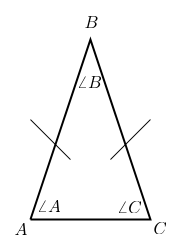
\includegraphics[scale=0.5]{img/tri.png}
\end{figure}
\end{teorema}
\begin{proof}

Si comincia la dimostrazione con l'elenco delle conoscenze pregresse:
\begin{enumerate}
\item se due triangoli sono uguali essi hanno lati e angoli uguali
\item se due triangoli hanno due lati e l'angolo sotteso uguale allora i due triangoli sono uguali
\item se viene definita la bisettrice di $\angle B$, $\overline{BH}$, si ha che $\angle ABH = \angle HBC$
\begin{figure}
\centering
\caption{Triangolo isoscele scomposto in due triangoli rettangoli}
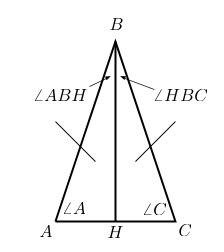
\includegraphics[scale=0.5]{img/tri2.png}
\end{figure}

\end{enumerate}
Procediamo ora coi passi della dimostrazione:
\begin{enumerate}
\item $\overline{AB}=\overline{BC}$ per ipotesi
\item $\angle ABH = \angle HBC$ per la terza conoscenza pregressa
\item $HBC = ABH$ per la seconda conoscenza pregressa in quanto due lati sono uguali per ipotesi e dal passo precedente
      l'angolo sotteso ai due lati uguali è uguale in ambedue i triangoli.
\item $\angle A= \angle C$ per la prima conoscenza pregressa dato che $HBC = ABH$
\end{enumerate}
Siamo così giunti alla fine della dimostrazione ma adesso vogliamo rappresentarla attraverso gli strumenti della logica al fine di renderla
totalmente formale per cui si effettua i seguenti passaggi:
\begin{itemize}
\item si è trasformata la seconda conoscenza pregressa in:\newline
  \textbf{se} $\overline{AB}=\overline{BC}$ \textbf{e} $\overline{BH}=\overline{BH}$ \textbf{e} $\angle ABH = \angle HBC$
  \textbf{allora} $ABH = HBC$
\item si è trasformata la prima conoscenza pregressa in:\newline
  \textbf{se} $ABH = HBC$ \textbf{allora} $\overline{AB}=\overline{BC}$ \textbf{e} $\overline{BH}=\overline{BH}$
  \textbf{e} $\overline{AH}=\overline{HC}$ \textbf{e} $\angle ABH = \angle HBC$ \textbf{e} $\angle AHB = \angle CBH$ \textbf{e} $\angle A=\angle C$
\end{itemize}
Possiamo ora procedere col processo di formalizzazione, ossia il processo che ci permette di affermare
$\overline{AB} = \overline{BC} \vdash \angle A = \angle C$ con $\vdash$ simbolo di derivazione logica.

Assumendo $P = \{ \overline{AB} = \overline{BC}, \angle ABH = \angle HBC, \overline{BH} = \overline{BH} \}$
ed avendo le seguenti conoscenze pregresse:
\begin{enumerate}
\item $\overline{AB}=\overline{BC} \land \overline{BH}=\overline{BH} \land \angle ABH = \angle HBC \rightarrow  ABH = HBC$
\item $ABH = HBC \rightarrow \overline{AB}=\overline{BC} \land \overline{BH}=\overline{BH} \land \overline{AH}=\overline{HC}
        \land \newline \angle ABH = \angle HBC \land \angle AHB = \angle CBH \land \angle A=\angle C$.
\end{enumerate}
per ottenere $\overline{AB} = \overline{BC} \vdash \angle A = \angle C$ bisogna effettuare la seguente catena:
\begin{description}
\item [P1] $\overline{AB}=\overline{BC}$  da \textbf{P}
\item [P2] $\angle ABH = \angle HBC$  da \textbf{P}
\item [P3] $\overline{BH}=\overline{BH}$  da \textbf{P}
\item [P4] $\overline{AB} = \overline{BC} \land \overline{BH} = \overline{BH} \land \angle ABH = \angle HBC$
       da \textbf{P1, P2, P3} attraverso l' \textbf{introduzione della congiunzione}.
\item [P5] $ABH = HBC$ da \textbf{P4}, dalla \textbf{regola 2}  attraverso l'applicazione del \textbf{modus ponens}.
\item [P6] $\overline{AB} = \overline{BC} \land \overline{BH} = \overline{BH} \land \overline{AH} = \overline{HC} \land \newline
  \angle ABH = \angle HBC \land \angle AHB = \angle CBH \land \angle A=\angle C$ da \textbf{P5}, dalla \textbf{regola 1} attraverso Modus Ponens.
\item [P7] $\angle A=\angle C$ da \textbf{P6} attraverso \textbf{eliminazione della congiunzione}
\end{description}
\end{proof}
\begin{defi}
  Una dimostrazione, chiamata \textbf{dim}, indicata con $S\,\,\vdash\,\, F$, è un sequenza:
\begin{equation*}
  dim=<P_1,P_2,...,P_n>
\end{equation*}
con:
\begin{itemize}
\item $P_n=F$
\item $P_i \in S$ o con $P_i$ ottenibile dalle $P_1,...,P_{i-1}$ applicando una regola di inferenza
\end{itemize}
\end{defi}
Un insieme di regole di inferenza costituisce la base di un calcolo logico, il quale ha lo scopo di manipolare le formule in modo
unicamente sintattico al fine di stabilire una connessione tra un insieme di formule di partenza, dette assiomi e un insieme di conclusioni.

\section{Logica Proporzionale}
La logica proposizionale si occupa delle conclusioni che si possono trarre da un insieme di proposizioni,
ma purtroppo è un linguaggio limitato in quanto non si può generalizzare le proposizioni e/o definire delle proprietà.

La sintassi di un linguaggio è composta da una serie di formule ben formate($FBF$) definite induttivamente nel seguente modo:
%definizione formule ben formate
\begin{enumerate}
  \item Le costanti e le variabili proposizionali sono $FBF$.
  \item Se $A$ e $B$ sono $FBF$ allora $(A \land B)$,$(A \lor B)$,$(\neg A)$,$(A \rightarrow B)$,
        $TA$ e $FA$ sono delle formule ben formate.
  \item nient'altro è una formula
\end{enumerate}

Esempio:\newline
$(P \land Q) \in Fbf$  è una formula ben formata\newline
$(PQ \land R) \not \in Fbf$ in quanto non si rispetta la sintassi del linguaggio definita.\newline

La semantica di una logica consente di dare un significato e un interpretazione alle formule del Linguaggio.\newline
\begin{defi}
  Sia data una formula proposizionale $P$ e sia ${P_1,\dots,P_n}$, l'insieme degli atomi che compaiono nella formula $A$.\newline
  Si definisce come \emph{interpretazione} una funzione $v:\{P_1,\dots,P_n\} \mapsto \{T,F\}$ che attribuisce un valore di verità
  a ciascun atomo della formula $A$.
\end{defi}
I connettivi della Logica Proposizionale hanno i seguenti valori di verità:
%Tabella di Verità degli operatori
\begin{table}
$\begin{array}{cccccc}
\toprule
\text{A} & \text{B} & A \land B & A \lor B & \neg A & A \rightarrow B\\
\midrule
    F & F & F & F & T & T\\
    F & T & F & T & T & T\\
    T & F & F & T & F & F\\
    T & T & T & T & F & T\\
\bottomrule
\end{array}$
\end{table}
La tavola di verità costituisce la semantica di un insieme di proposizioni mentre un calcolo logico dice come generare nuove formule logiche,
ovvero espressioni sintattiche, a partire dagli assiomi e questo processo di generazione si chiama dimostrazione.

Per ottenere nuove formule dagli assiomi si usa il calcolo proposizionale, che si base sulle regole di inferenza, ossia regole attraverso
cui si può derivare una nuova formula ben formata.\newline
Le regole di inferenza analizzate sono le seguenti:
\begin{itemize}
\item \textbf{Modus Ponens:}
  \begin{equation*}
    \frac{a\to b,\,\,a}{b}
  \end{equation*}
\item \textbf{Modus Tollens:}
  \begin{equation*}
    \frac{a\to b, \neg b}{\neg a}
  \end{equation*}
\item \textbf{Eliminazione $\land$:}
  \begin{equation*}
    \frac{P_1\land P_2 \land ... \land P_n}{P_i}\,\,
  \end{equation*}
\item \textbf{Introduzione di $\land$}:
  \begin{equation*}
    \frac{P_1, P_2,...,P_n}{P_1\land P_2 \land ... \land P_n}\,\,
  \end{equation*}
\item \textbf{Introduzione di $\lor$:}
  \begin{equation*}
    \frac{a}{a \lor b}
  \end{equation*}
\item \textbf{Terzo Escluso:}
  \begin{equation*}
    \frac{a \lor \neg a}{vero}
  \end{equation*}

\item \textbf{Eliminazione di $\neg$}:
  \begin{equation*}
    \frac{\neg \neg a}{a}
  \end{equation*}

\item \textbf{Eliminazione di $\land$}:
  \begin{equation*}
    \frac{a \land vero}{a}
  \end{equation*}
\item \textbf{Contraddizione:}
  \begin{equation*}
    \frac{a \land \neg a}{b}
  \end{equation*}
ovvero da una contraddizione posso trarre qualsiasi conseguenza
\end{itemize}
Queste regole di inferenza fanno parte del calcolo naturale, detto anche di Gentzen, similare al calcolo tramite Tableaux visto nel corso
di Fondamenti dell'informatica.\newline
Questo tipo di calcolo consiste nel formalizzare i modi di derivare conclusioni a partire dalle premesse, ovvero di derivare direttamente un FBF
mediante una sequenza di passi ben codificati.\newline
La regola del modus ponens  insieme al principio del terzo escluso, posso essere usati anche procedendo per assurdo alla dimostrazione
di una data formula e ciò viene detto \emph{principio di risoluzione}, affrontata poi quando analizziamo il linguaggio Prolog.

Una formula nella logica proposizionale può essere di 4 diversi tipi:
%Tipologie di formule
\begin{description}
    \item[tautologica] la formula è soddisfatta da qualsiasi valutazione della formula.
    \item[soddisfacibile non tautologica] la formula è soddisfatta da qualche valutazione.
    \item[falsibicabile] la formula non è soddisfatta da qualche valutazione della formula.
    \item[contraddizione] la formula non viene mai soddisfatta.
\end{description}

La logica proposizionale è decidibile, ossia posso sempre verificare il significato di una formula, infatti esiste
una procedura effettiva che stabilisce la validità o no di una formula, o se questa ad esempio è una tautologia.\newline
In particolare il verificare se una proposizione è tautologica o meno è l’operazione di decibilità principale che si svolge
nel calcolo proposizonale.

Una dimostrazione di una formula di una logica può venire tramite:
\begin{itemize}
  \item  \textbf{Metodo diretto}: Data un'ipotesi, attraverso una serie di passi
          si riesce a dimostrare la correttezza della Tesi
  \item \textbf{Metodo per assurdo}(non sempre accettato in tutte le logiche):
        Si nega la tesi ed attraverso una serie di passi si riesce a dimostrare
        la negazione delle ipotesi.
\end{itemize}

La logica proposizionale è completa e corretta per cui data una formula ben formata, sia utilizzando i sistemi deduttivi sia analizzando
la semantica, si è in grado di stabilire se una formula è tautologica, soddisfacibile o falsificabile.

\section{Logica del primo ordine}
La logica del primo ordine, chiamata anche logica predicativa, permette di quantificare i vari fatti ed introduce il concetto di funzione e
predicato per poter esprimere delle proprietà su una serie di individui.

Un linguaggio predicativo $L$ è composto dai seguenti insiemi di simboli:
\begin{enumerate}
    \item insieme di variabili individuali(infiniti) $x,y,z,\dots$
    \item connettivi logici: $\land \lor \neg \rightarrow \iff$
    \item quantificatori: $\forall \exists$
    \item simboli: ( , )
    \item Costanti proposizionali: $T,F$
    \item simbolo di uguaglianza $=$, eventualmente assente
\end{enumerate}
Questa è la parte del linguaggio tipica di ogni linguaggio del primo ordine poi ogni linguaggio definisce la propria segnatura:
\begin{enumerate}
    \item insiemi di simboli di costante $a,b,c,\dots$
    \item simboli di funzione con arieta $f,g,h,\dots$
    \item simboli di predicato $P,Q,Z,\dots$ con arietà
\end{enumerate}

%Esempio
Esempio:Linguaggio della teoria degli insiemi \newline
Costante:$\emptyset$\newline
Predicati:$\in(x,y)$, $=(x,y)$

Esempio:Linguaggio della teoria dei Numeri \newline
Costante:$0$ \newline
Predicati:$<(x,y)$,$=(x,y)$ \newline
Funzioni:$succ(x)$,$+(x,y)$,$*(x,y)$

%Definizione di Termini e Formule ben formate
Per definire le formule ben formate della logica predicativa bisogna prima definire
l'insieme di termini e le formule atomiche.
\begin{defi}
    L'insieme $TERM$ dei termini è definito induttivamente come segue
    \begin{enumerate}
        \item Ogni variabile e costante è un termine
        \item Se $t_1 \dots t_n$ sono dei termini e $f$ è un simbolo di funzione di arietà $n$
              allora $f(t_1,\dots,t_n)$ è un termine
    \end{enumerate}
\end{defi}
%Inserire esempi
\begin{defi}
    L'insieme $ATOM$ delle formule atomiche è definito come:
    \begin{enumerate}
        \item $T$ e $F$ sono degli atomi
        \item Se $t_1$ e $t_2$ sono dei termini, allora $t_1 = t_2$ è un atomo
        \item Se $t_1,\dots,t_n$ sono dei termini e $P$ è un predicato a $n$ argomenti,
              allora $P(t_1,\dots,t_n)$ è un atomo.
    \end{enumerate}
\end{defi}
%Inserire esempi
\begin{defi}
    L'insieme delle formule ben formate($FBF$) di $L$ è definito induttivamente come
    \begin{enumerate}
        \item Ogni atomo è una formula
        \item Se $A,B \in FBF$, allora $\neg A$, $A \land B$,$A \lor B$,$A \rightarrow B$
              e $A \iff B$ appartengono alle formule ben formate
        \item Se $A \in FBF$ e $x$ è una variabile, allora $\forall x A$ e $\exists x A$
              appartengono alle formule ben formate
        \item Nient'altro è una formula
    \end{enumerate}
\end{defi}
%Inserire esempi

%Variabili legate e chiuse
\begin{defi}
    L'insieme $var(t)$ delle variabili di un termine $t$ è definito come segue:
    \begin{itemize}
        \item $var(t) = \{t \}$, se $t$ è una variabile
        \item $var(t) = \emptyset$ se $t$ è una costante
        \item $var(f(t_1,\dots,t_n)) = \bigcup _{i = 1} ^n var(t_i)$
        \item $var(R(t_1,\dots,t_n)) = \bigcup _{i = 1} ^ n var(t_i)$
    \end{itemize}
\end{defi}
Si definisce come \emph{aperto} un termine che non contiene variabili altrimenti il termine è \emph{chiuso}.\newline
Le variabili nei termini e nelle formule atomiche possono essere soltanto libere
in quanto gli unici operatori che "legano" le variabili sono i quantificatori.

Il campo di azione dei quantificatori si riferisce soltanto alla parte in cui si applica il quantificatore per cui
una variabile si dice \emph{libera} se non ricade nel campo di azione di un quantificatore altrimenti è \emph{vincolata}.

Si aggiunge una nuova regola d'inferenza per la logica dei predicati, l'eliminazione del quantificatore universale $\forall$:
\begin{equation*}
  \frac{\forall x, T(...,x,...), c\in C}{T(...,c,...)}
\end{equation*}

Abbiamo altre regole di inferenza per il quantificatore esistenziale:
\begin{itemize}
\item \textbf{Introduzione del quantificatore esistenziale $\exists$}:
  \begin{equation*}
    \frac{T(...,c,...), c\in C}{\exists x, T(...,x,...)}
  \end{equation*}
\item si hanno le seguente identità:
  \begin{equation*}
    \begin{split}
      \exists x, \neg T(...,x,...)\equiv \neg\forall x, T)...,x,...) \\
      \forall x, \neg T(...,x,...)\equiv \neg\exists x, T(...,x,...)\\
    \end{split}
  \end{equation*}
\end{itemize}
Per una trattazione migliore e per approfondimenti sulla logica si può consultare gli appunti del corso di Fondamenti oppure i vari libri di
logica, come ad esempio ``How to prove it''.
%Capitolo sulla logica matematica
%Capitolo sulla programmazione in Prolog
\chapter{Programming in Logic}
Dopo aver effettuato un ripasso della logica, incominciamo a considerare il Prolog e la programmazione logica:
le basi sono state poste da Robert Kowalski e Marten Van Emdem, mentre la progettazione e implementazione,
avvenne nel 1972 a Marsiglia grazie ad Alain Colmerauer e Philippe Roussel.

Il Prolog è un linguaggio di programmazione logica basato sulle clausole di Horn, la cui definizione sarà data in seguito,
e la procedura utilizzata dal Prolog per la computazione è il principio di risoluzione e di unificazione, anch'esso trattato in seguito.

Un programma logico è formato da un insieme di istruzioni, rappresentanti un sottoinsieme di frasi ben formate della logica del primo ordine
e l'ambiente Prolog determina se una data assunzione è verificata o meno nel programma e sotto quali eventuali vincoli.

I componenti basilari di un programma Prolog, rappresentanti tutti una clausola di Horn, sono:
\begin{description}
\item [Fatti]: indica una relazione esistente tra due oggetti, necessaria per stabilire la base di conoscenza del linguaggio.
               \begin{minted}{prolog}
                 worksFor(paolo, coop).
               \end{minted}
\item [Query]: chiede al sistema l'esistenza di una relazione tra gli oggetti e quindi inizia una deduzione per stabilire se la query
               è una conseguenza diretta del programma, dopo l'applicazione del principio di risoluzione per un numero finito di volte.
               \begin{minted}{prolog}
                 :- worksFor(paolo, trenord).
               \end{minted}

\item [Regole]: definisce una nuova relazione esistente tra gli oggetti, ossia permette di derivare una nuova conclusione dalla base di conoscenza.
                \begin{minted}{prolog}
                  parent(X, Y) :- father(X, Y).
                \end{minted}
                La testa della regola $A$, viene detta conseguenza mentre il corpo $B_1, B_2, \dots, B_n$ sono l'antecedente
                e il simbolo :- indica il simbolo logico di implicazione.\newline
                Una relazione può essere definita ricorsiva, per cui necessita di almeno due regole, una per il caso base e
                una per il caso passo, come il seguente esempio:
                \begin{minted}{prolog}
                    natural_number(0).
                    natural_number(s(X)) :- natural_number(X).%s(X) indica il successore di X
                \end{minted}
\end{description}
I fatti e le regole sono quantificate universalmente mentre una query si intende sempre quantificata esistenzialmente, per cui una query
risponde true se esiste un instanza $\alpha$ che la verifica altrimenti risponde false.

Le query e le regole le abbiamo definite nella forma generale, ossia possiamo definire regole e query su congiunzioni di termini,
infatti il simbolo \textbf{``,''} rappresenta l'operatore logico and, perciò in caso più termini hanno lo stesso simbolo di variabile
l'instanza $\alpha$ deve essere la stessa per stabilire se una query è una conseguenza diretta del programma.

Per vedere al meglio il concetto di implicazione vediamo la definizione del concetto di nonno nel linguaggio Prolog:
\begin{minted}{prolog}
  grandfather(X, Y) :- father(X, Z), parent(Z, Y).
\end{minted}
Questa relazione stabilisce che X è il nonno di Y se risulta che esiste un Z tale che X è padre di Z e Z è genitore di Y.

Ogni espressione prolog viene chiamata \emph{termine}, che può essere della seguente tipologia:
\begin{description}
\item [atomi] : elemento base del Prolog rappresentato da un numero, qualsiasi sequenza racchiusa tra ' ',
       una sequenza di caratteri alfanumerici, con la lettera minuscola iniziale, e nel SWI-Prolog anche una stringa indica un atomo.

\item [variabili] : sequenza di caratteri alfanumerici, iniziata con la lettera maiuscola oppure con \_ e vengono inizializzate
                    quando il sistema prova a dimostrare una query.\newline
                    Una variabile composta soltanto dal simbolo \_ viene detta \emph{anonima}.

\item [termini composti]: indicato da un funtore, simbolo usato per il nome di una funzione/predicato, e da una sequenza
  di termini all'interno di parentesi e separati da una virgola, usati per rappresentare gli argomenti del funtore.
\end{description}

Un programma caricato nel sistema prolog rappresenta una base di conoscenza, mostrabile nei seguenti modi:
\begin{itemize}
\item tutte le informazioni vengono rappresentate come argomenti in un'unica relazione e ciò può essere comodo solo per
  piccole relazioni dato che è difficile da mantenere e coprendere una relazione così definita.
  %inserire esempio
\item le informazioni vengono rappresentate con più relazione annidate tra di loro e ciò aumenta la leggibilità e
  la mantenibilità del programma prolog.
 %Inserire esempio
\item tutte le relazioni possono essere rappresentate tramite lo schema XML
\end{itemize}
Per riuscire a stabilire se un goals è una conseguenza diretta del programma il sistema prolog utilizza il principio di risoluzione,
utilizzato per effettuare la dimostrazione del programma , e il principio di unificazione, necessario come si evince dal nome per
unificare le variabili presenti in una formula del programma.

Nei prossimi due paragrafi considereremo questi due principi al fine di comprendere al meglio come avviene la computazione in un linguaggio logico.
\section{Principio di Risoluzione}
Il principio di risoluzione è una regola di inferenza generalizzata semplice e facilmente implementabile in un calcolatore
ed opera su formule ben formate nella forma normale congiuntiva, in cui i letterali si chiamano clausole.\newline
Questo principio viene utilizzato  per la dimostrazione di formule ben formate attraverso la refutazione per assurdo,
metodologia usata dall'interprete Prolog per computare una data query.

La regola di inferenza ha la seguente forma:
\begin{equation*}
  \frac{p\vee r,\, s\lor \neg r}{p\vee s}\,\,\,\,\,\,\,\,\,\,\frac{\neg r,\, r}{\perp}
\end{equation*}
dove:
\begin{itemize}
\item $p \lor  s$ è la \textit{clausola risolvente}
\item $\perp$ è la \textit{clausola vuota}, che corrisponde all'aver creato una contraddizione da cui posso dedurre qualsiasi cosa,
       compresa anche la clausola vuota.
\end{itemize}
Vediamo un'altra regola di inferenza, la\textbf{unit resolution}:
   \begin{equation*}
     \frac{\neg p,\,\, q_1\vee q_2\vee ... \vee q_k \vee p}{q_1\vee q_2\vee ... \vee q_k}
   \end{equation*}
o anche:
\begin{equation*}
  \frac{p,\,\, q_1\vee q_2\vee ... \vee q_k \vee \neg p}{q_1\vee q_2\vee ... \vee q_k}
\end{equation*}
è una regola di risoluzione molto generale, chiamata anche procedura di Davis-Putnam, e se una delle due clausole da risolvere
è un \textit{letterale} si parla di \emph{unit resolution}.\newline
Come esempio si può avere:
\begin{itemize}
\item non piove, piove e c'è il sole
\item si desume quindi che c'è il sole
\end{itemize}

Ogni FBF può essere in \emph{forma normale a clausola}:
\begin{itemize}
\item \emph{formula normale congiunta:} congiunzione di disgiunzioni o di negazione di predicati (sia positivi che negativi):
  \begin{equation*}
    \bigwedge_i(\bigvee_iL_{ij})
  \end{equation*}
\begin{esempio}
ecco degli esempi:
\begin{itemize}
\item $(p(x)\lor q(x,y)\lor \neg t(z))\land(p(w)\lor \neg s((u)\lor \neg r(v))$
\item $(\neg t(z))\lor (p(w)\lor \neg s(u))\land (p(x)\lor s(x)\lor q(y))$
\end{itemize}
\end{esempio}

\item \textit{forma normale disgiunta}: disgiunzione di congiunzioni o di negazione di predicati (sia positivi che negativi)
  \begin{equation*}
    \bigvee_i(\bigwedge_j L_{ij})
  \end{equation*}
\end{itemize}
Le clausole con un solo letterale positivo solo le \textit{clausole di Horn}, con lo presenza o meno di letterali negativi,
usate per rappresentare tutti i termini delle formule in Prolog.\newline
Ovviamente non tutte le formule ben formate possono essere rappresentate tramite le clausole di Horn per cui il Prolog è un sottoinsieme
della logica del Primo Ordine.\newline
Attraverso questa restrizione nel 1974 Kowalski produsse un interpretazione procedurale delle dimostrazione e ciò diventò la base
della semantica del Prolog.
%Semantica in Prolog
\section{Principio di Unificazione}
Il principio di unificazione è il cuore del modello di computazione dei programmi logici ed è alla base della deduzione automatica
e dell'uso dell'inferenza logica nell'intelligenza artificiale.

Per poter definirlo dobbiamo introdurre le seguenti definizioni:
\begin{defi}
Un termine $t$ è un instanza comune  di $t_1$ e $t_2$ se esistono le sostituzioni $\alpha_1$ e $\alpha_2$
che rendono $t$ uguale a $\alpha_1t_1$ e a $\alpha_2t_2$.\newline
Un termine $s$ è un termine generale del termine $t$ se $t$ è un'istanza di $s$ ma $s$ non è un istanza di $t$.\newline
Un termine $s$ è una variante alfabetica del termine $t$ se $t$ è un istanza di $s$ e $s$ è un istanza di $t$.
\end{defi}
L'unificazione tra due termini consiste nell'effettuare una sostituzione che rende i due termini identici
per cui c'è una relazione chiusa con l'instanza comune di due termini.

Il principio di unificazione consiste nel trovare il \emph{mgu}(Most general unifier),
l'unificazione la cui instanza comune è un termine generale, e in caso non lo trova riporta un fallimento.\newline
Presentiamo ora alcuni esempi per capire come funziona il Mgu:
\begin{minted}{prolog}
Mgu(42, 42) % ->{} non serve nessuna sostituzione
Mgu(42, X) % ->{X/42} ovvero X deve essere 42
Mgu(X,42) % ->{X/42} ovvero X deve essere 42
Mgu(foo(bar, 42), foo(bar, X)) % ->{X/42} ovvero X deve essere 42
Mgu(foo(Y, 42), foo(bar, X)) % ->{Y/bar, X/42} ovvero X deve essere 42
Mgu(foo(bar(42), baz), foo(X, Y))  /* ->{X/bar (42), Y/baz}
 ovvero X deve essere  bar(42) e Y baz*/
Mgu(foo(X), foo(bar(Y)))
Mgu(foo(bar(42), baz), foo(X, Y))  /* ->{X/bar (y), Y_:G001}
 ovvero non si ha soluzione */
\end{minted}
L'Mgu non è altro che il risultato finale della procedura di valutazione del Prolog ed il modo più semplice per vedere
se l'unificazione è corretta effettuiamo le seguenti interrogazioni al sistema Prolog:
\begin{minted}{prolog}
?- 42 = 42.
Yes

?- 42 = X.
X = 42 % per rendere vera l'affermazione serve x = 42
Yes

?- foo(bar, 42) = foo(bar, X).
X = 42
Yes

?- foo(Y, 42) = foo(bar, X).
Y = bar
X = 42
Yes

?- foo(bar(42), baz) = foo(X, Y).
X = bar(42)
Y = baz
Yes

?- foo(X) = foo(bar(Y)).
X = bar(Y)
Y = _G001
Yes

?- foo(42, bar(X), trillian) = foo(Y, bar(Y), X).
No
\end{minted}

Vediamo ora un programma che effettua la somma tra due numeri naturali:
\begin{minted}{prolog}
sum(0, X, X).
sum(s(X), Y, s(Z)) -: sum(X, Y, Z).
\end{minted}
con $s(n)$ interpretato come il successore ($0=0,\, s(0)=1, \,s(s(0))=2,\dots $).\newline
Quando viene specificato un goal esso viene confrontato con tutte le clausole di programma, che usa il procedimento di negazione
e di trasformazione in sintassi Prolog come viene mostrato in dettaglio con questo esempio:
\begin{itemize}
\item  interroghiamo il programma:
  \begin{equation*}
  \begin{split}
    \exists X\,\,\, sum(s(0),\, 0,\, X)\,\,\,\,\,\{X\,/\, s(0)\} \\
    \exists W\,\,\, sum(s(s(0)),\, s(0), \, W)\,\,\,\,\,\{W\,/\, s(s(s(0)))\}
  \end{split}
  \end{equation*}
dove $\{X\,/\, s(0)\}$ e $\{W\,/\, s(s(s(0)))\}$ sono le sostituzioni che rappresentano il risultato
\item usiamo il procedimento di negazione e trasformazione in sintassi:
\begin{minted}{prolog}
:- sum(s(0), 0, N).    %{N / s(0)}
:- sum (s(s(0)), s(0), W).     %{W / s(s(s(0)))}
\end{minted}
con $\{N\, /\, s(0)\}$ e $\{W \,/\, s(s(s(0)))\}$ che sono le sostituzioni.
\end{itemize}
Una computazione corrisponde al tentativo di dimostrare, tramite la regola di risoluzione, che una formula segue logicamente da un programma
e si ha inoltre che si deve determinare una sostituzione per le variabili del goal per cui la query segue  logicamente dal programma:
\begin{esempio}
Sia dato il programma P e la query:
\begin{minted}{prolog}
:- p(t1, t2, ..., tm).
\end{minted}
se \textbf{X1,..., Xn} sono le variabili in \textbf{t1,..., tm}, il significato della query è:
\begin{equation*}
  \exists X1,\,..., \,Xn\, . \,p(t1, t2, ..., tm)
\end{equation*}
e si cerca una sostituzione:
\begin{equation*}
  s=\{X1\,/\,s1,...,\, Xn\,/\,sn\}
\end{equation*}
con gli $s\,i$ termini tali per cui:
\begin{equation*}
  P\vdash s[p(t1, t2, ..., tm)]
\end{equation*}
\end{esempio}
Dato un insieme di clausole di Horn è possibile derivare la clausola vuota solo se c'è almeno una clausola senza testa, ovvero una query $G_0$
, in cui si deve dimostrare che da $P \cup G_0$ si può derivare la clausola e ciò avviene per assurdo col principio di risoluzione.\newline
Nel prossimo paragrafo vediamo come effuttua la risoluzione il sistema Prolog, che per efficienza usa una forma particolare di risoluzione.
\subsection{Risoluzione ad Input Lineare (SLD)}
Come già visto, il sistema Prolog per dimostrare la veridicità di un goal esegue una sequenza di passi di risoluzione,
il cui ordine di esecuzione determina sistemi di prova più o meno efficienti.\newline
In Prolog la risoluzione avviene sempre fra l’ultimo goal derivato in ciascun passo e una clausola di programma
e questa forma è detta \emph{Risoluzione-SLD}, dove le sentenze lineari sono le clausole di Horn.
\begin{defi}
Partiamo dal goal $G_i$:
\begin{equation*}
  G_i\equiv \,\,\,?-\, A_{i,\, 1}, ...,  A_{i,\, m}.
\end{equation*}
e dalla regola:
\begin{equation*}
  A_r\,\,\,:-\,\,\, B_{r,\,1},..., B_{r,\,k}.
\end{equation*}
Se esiste un unificatore $\sigma$ tale che $\sigma[A_r]=\sigma[A_{i,\,1}]$ allora si ottiene il nuovo goal:
\begin{equation*}
  G_{i+1}\equiv\,\,\,B^{'}_{r,\,1},..., B^{'}_{r,\,k},A^{'}_{i,\, 1}, ...,  A^{'}_{i,\, m}.
\end{equation*}
che è un passo di risoluzione eseguito dal sistema Prolog (con $\sigma[A_{i,\,m}]=A^{'}_{i,\,m}$ 4 $\sigma[B_{i,\,m}]=B^{'}_{i,\,m}$.\newline
La scelta di unificare il primo sottogoal di $G_i$ è arbitraria infatti si sarebbe potuto scegliere un arbitario sottogoal di $G_i$.

Partiamo dal goal $G_i$:
\begin{equation*}
  G_i\equiv \,\,\,?-\, A_{i,\, 1}, ...,  A_{i,\, m}.
\end{equation*}
e dalla regola (ovvero dal \textbf{fatto}): $A_r$.
se esiste un unificatore $\sigma$ tale che $\sigma[A_r]=\sigma[A_{i,\,1}]$ allora si ottiene il nuovo goal:
\begin{equation*}
  G_{i+1}\equiv\,\,\,A^{'}_{i,\, 2}, ...,  A^{'}_{i,\, m}.
\end{equation*}
che ha dimensioni minori di $G_i$ avendo $m-1$ sottogoal
\end{defi}
Nella risoluzione SLD si possono avere i seguenti risultati:
\begin{itemize}
\item \textbf{successo:} si genera la clausola vuota, ovvero se per $n$ finito $G_n$ è uguale alla clausola vuota $G_:n\equiv\,\,\,:-$
\item \textbf{insuccesso finito}: se per $n$ finito $G_n$  non è uguale alla clausola vuota $G_:n\equiv\,\,\,:-$
              e non è più possibile derivare un nuovo \textit{risolvente} da $G_n$ ed una clausola d programma.
\item \textbf{insuccesso infinito: }se è sempre possibile derivare nuovi risolventi tutti diversi dalla clausola vuota.
\end{itemize}
La \textbf{sostituzione di risposta} è la sequenza di unificatori usati ed applicata alle variabili nei termini del goal iniziale
determina la risposta finale restituita dal sistema Prolog.\newline
Durante il processo di generazione di goal intermedi si costruiscono delle varianti dei letterali e delle clausole coinvolti
mediante larinominazione di variabili infatti una variante per una clausola $C$ é la clausola $C^{'}$ ottenuta da $C$ rinominando le sue variabili
\begin{esempio}
esempio:
\begin{minted}{prolog}
p(X) :- q(X, g(Z)).
% è uguale alla clausola con variabili rinominate:
p(X1) :- q(X1, g(FooFrobboz)).
\end{minted}
\end{esempio}
Possono esserci più clausole di programma utilizzabili per applicare la risoluzione con il goal corrente ed esistono diverse strategie di ricerca:
\begin{itemize}
\item \textbf{in profondità (Depth First)}: si sceglie una clausola e si mantiene fissa questa scelta, finché non si arriva alla clausola vuota
  o alla impossibilità di fare nuove risoluzioni: in questo ultimo caso si riconsiderano le scelte fatte precedentemente e si riparte a dimostrare
  in profondità fino a quando è possibile effettuare delle scelte.
\item \textbf{in ampiezza (Breadth First)}: si considerano in parallelo tutte le possibili alternative
\end{itemize}
Ogni sistema di programmazione logica sceglie la propria strategia e il Prolog ha deciso di adottare una strategia di risoluzione
in profondità con backtracking, ossia la possibilità di ritornare indietro e provare tutte le possibilità.

Introduciamo ora l'importante argomento degli alberi di derivazione, per analizzare come un sistema Prolog effettua la computazione
e quali passi esegue per riuscire a stabilire se una data query deriva dal programma o meno.
\begin{defi}
Dato un programma logico $P$, un goal $G_i$ e una regola di calcolo $R$ si ha che un \textit{albero SLD} per $P\cup G_i$ via $R$
è definito sulla base del processo di prova visto precedentemente:
\begin{itemize}
\item ciascun \textbf{nodo} dell'albero è un goal (possibilmente vuoto)
\item la \textbf{radice }dell'albero SLD è il goal $G_0$
\item dato il nodo: $:-\,\,\, A_1,...,A_{m-1},A_m,A_{m+1},...,A_k$
  se $A_m$ è il sottogoal selezionato dalla regola di calcolo $R$, allora questo nodo (genitore) ha un nodo figlio
  per ciascuna clausola del tipo:
  \begin{equation*}
    \begin{split}
      C_i\equiv A_i\,\,\, :-\,\,\, B_{i,\,1},...,B_{i,\,q}\\
      C_k \equiv A_k \\
    \end{split}
  \end{equation*}
di $P$ tale che $A_i$ e $A_m$ ($A_K$ e $A_m$) sono unificabili attraverso la sostituzione più generale $\sigma$.\newline
Il nodo figlio è etichettato con la clausola goal
\begin{equation*}
\begin{split}
      :-\,\,\,\sigma[A_1,...,A_{m-1},B_{i,\,i},...,B_{i,\,q},A_{m+1},...,A_k]\\
      :-\,\,\,\sigma[A_1,...,A_{m-1},A_m,A_{m+1},...,A_k]\\
\end{split}
\end{equation*}
e il ramo dal nodo padre al figlio è etichettato dalla sostituzione $\sigma$ e dalla clausola selezionata $C_i$ o $C_k$
ed infine si ha che il nodo $:-$ non ha figli.
\end{itemize}
\end{defi}
La regola $R$ è variabile e le più comuni utilizzate sono:
\begin{itemize}
\item \textbf{Left-most}: si sceglie sempre di risolvereil sottogoal più a sinistra
\item \textbf{Right-most}: si sceglie sempre la risoluzione del sottogoal più a destra
\item si può avere la scelta di un sottogoal a caso
\item se si ha un modo per decider il miglior sottogoal
\end{itemize}
Ogni sistema logico decide la propria modalità di applicazione della regola e il sistema Prolog ha deciso di
usare sempre la regola left-most.\newline
L'albero SLD, generato implicitamente dal sistema Prolog, ordina i figli di un nodo secondo l'ordine dall'alto verso il basso
delle regole e dei fatti del programma P, come si nota nell'esempio mostrato di seguito.
\begin{esempio}
Ecco un esempio:
\begin{center}
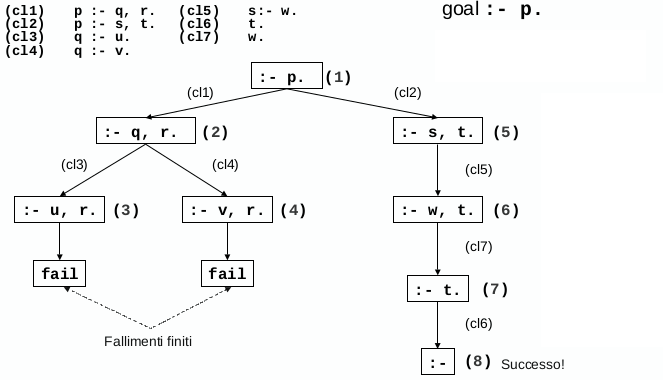
\includegraphics[scale=0.7]{img/alb.png}
\end{center}
\end{esempio}
Ad ogni ramo di un albero SLD corrisponde una derivazione SLD e ogni ramo che termina con il nodo vuoto $:-$.\newline
La regola di calcolo influisce sulla struttura dell'albero per quanto riguarda l'ampiezza e la profondità ma non influisce
sulla correttezza e completezza, infatti tra un albero left-most e un albero right-most cambia solo l'ordine e il tempo necessario
per stabilire se un ramo è un successo oppure no.
\begin{esempio}
  Ecco un altro esempio, con fallimento infinito, dove la clausola vuota può essere generata ma il Prolog non è in grado di trovare
  questa soluzione dato che la sua strategia di percorrimento dell’albero (implicito) di soluzioni è depth-first con backtracking :
\begin{center}
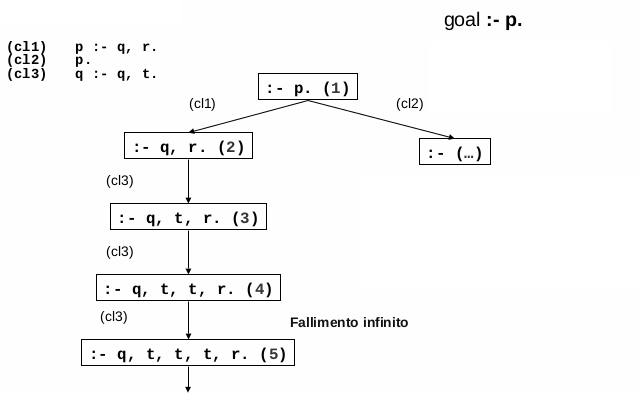
\includegraphics[scale=0.7]{img/alb2.png}
\end{center}
\end{esempio}
\subsection{Cut e Backtracking}
Introduciamo ora il predicato \emph{Cut}, attraverso cui possiamo controllare il backtracking, in quanto si tagliano certe possibilità
di ritornare indietro nelle scelte durante la computazione.\newline
Il predicato cut si indica con $!$ e il Prolog effettua un'interpretazione procedurale, sempre per il fatto che viene eseguito su un calcolatore.

Come abbiamo affermato precedentemente, le clausole nel data base di un programma Prolog vengono considerate “da sinistra, verso destra”
e “dall'alto al basso” per cui se un (sotto)goal fallisce, allora il dimostratore Prolog, sceglie un'alternativa,
scandendo “dall'alto” verso “il basso” la lista delle clausole.\newline
Questa procedurà può venire controllata dal \textit{cut} infatti per esempio:
\begin{minted}{prolog}
a :- b1, b2, ..., bk, !, ..., bn.
\end{minted}
Questo è l'effetto del cut:
\begin{itemize}
\item se il goal corrente \textit{G} unifica con \textit{a} e $b_1,...,b_k$ hanno successo,
      allora il dimostratore si impegna inderogabilmente alla scelta di C per dimostrare G.
\item ogni clausola alternativa (successiva, in basso) per \textit{a} che unifica con \textit{G} viene ignorata
\item se un qualche $b_j$ con $j > k$ fallisse, il backtracking si fermerebbe al cut e le altre scelte sono rimosse dall'albero di derivazione
\item quando il backtracking raggiunge il cut, allora il cut fallisce e la ricerca procede dall’ultimo punto di scelta
      prima che \textit{G} scegliesse \textit{C}
\end{itemize}
Il Prolog per la gestione della computazione utilizza due stack:
\begin{itemize}
\item stack delle scelte: contiene l'insieme delle scelte possibili ed ad ogni fase della valutazione contiene i puntatori alle
      scelte aperte nelle fasi precedenti della dimostrazione
\item stack di esecuzione: contiene i record di attivazione delle varie procedure, ovvero le sostituzioni per l'unificazione delle varie regole.
\end{itemize}
Vediamo un albero di derivazione in caso di cut:
\begin{center}
	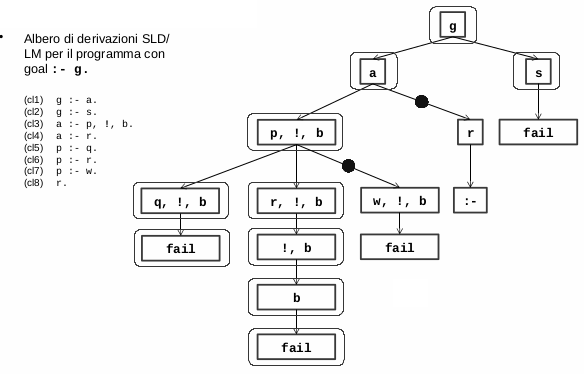
\includegraphics[scale=0.8]{img/cut.png}
\end{center}
Si hanno due tipi di cut:
\begin{itemize}
\item \textbf{green cut:} utili per esprimere il “determinismo”, come vedremo ora, e quindi per rendere più efficiente il programma
  in quanto non vengono analizzate clausole certamente false.
\item \textbf{red cut:} usati per soli scopi di efficienza ed hanno come caratteristica principale quella di omettere alcune condizioni
                        esplicite in un programma, ma soprattutto  quella di modificare la semantica del programma.
\end{itemize}
Per capire l'importanza e l'utilizzo del cut, consideriamo ora il seguente codice:
\begin{minted}{prolog}
/* merge di due liste ordinate*/

merge([X | Xs], [Y | Ys], [X | Zs]) :-
	X < Y,
	merge(Xs, [Y | Ys], Zs).
merge([X | Xs], [Y | Ys], [X, Y | Zs]) :-
	X = Y,
	merge(Xs, Ys, Zs).
merge([X | Xs], [Y | Ys], [Y | Zs]) :-
	X > Y,
	merge([X | Xs], Ys, Zs).
merge([], Ys, Ys).
merge(Xs, [], Xs).

/+ minimo tra due numeri */
minimum(X, Y, X) :- X =< Y.
minimum(X, Y, Y) :- Y < X.
\end{minted}
Vediamo cosa succede come computazione nell'interprete Prolog:
\begin{center}
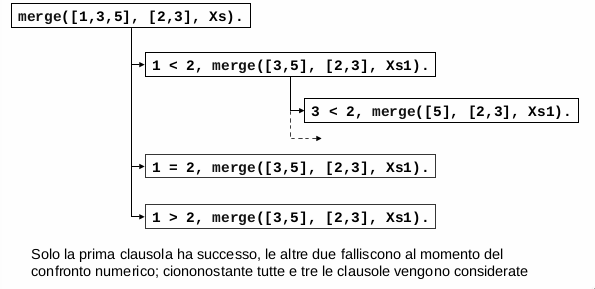
\includegraphics[scale=0.8]{img/cut2.png}
\end{center}
consideriamo la seguente query:
\begin{minted}{Prolog}
?- merge([], [], Xs).
Xs = [];
Xs = [];
False.
\end{minted}
Questa implementazione del merge ha purtroppo una soluzione di troppo e questo è un esempio di determinismo, ossia
quando una sola delle clausole serve (o si vorrebbe servisse) per provare un dato goal.\newline
Si usano quindi i seguenti green cuts:
\begin{minted}{prolog}
merge([X | Xs], [Y | Ys], [X | Zs]) :-
	X < Y, !,
	merge(Xs, [Y | Ys], Zs).
merge([X | Xs], [Y | Ys], [X, Y | Zs]) :-
	X = Y, !,
	merge(Xs, Ys, Zs).
merge([X | Xs], [Y | Ys], [Y | Zs]) :-
	X > Y, !,
	merge([X | Xs], Ys, Zs).
merge([], Ys, Ys) :- !.
merge(Xs, [], Xs) :- !.
\end{minted}
Interrogando il sistema Prolog come il seguente esempio otteniamo:
\begin{minted}{Prolog}
?- merge([], [], Xs).
Xs = [];
False.
\end{minted}
Guardando ai passi necessari, effettuati dall'interprete Prolog, per rispondere ad un query abbiamo:
\begin{center}
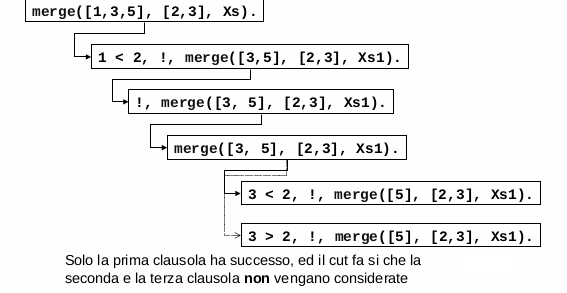
\includegraphics[scale=0.8]{img/cut3.png}
\end{center}
Il predicato per calcolare il minimo diventa:
\begin{minted}{prolog}
minimum(X, Y, X) :- X =< Y, !.
minimum(X, Y, Y) :- Y < X, !.%è ridontante ma viene inserito per simmetria
\end{minted}
Una volta che il programma ha fallito la prima clausola (ovvero il test X =< Y) al sistema Prolog non rimane che controllare la
clausola seguente.\newline
Riscrivo in maniera non simmetrica:
\begin{minted}{prolog}
minimum(X, Y, X) :- X =< Y, !.
minimum(X, Y, Y).
\end{minted}
Qui si ha un red cut dato che taglia solo delle soluzioni, portando anche a risultati errati, infatti $minimum(2, 5, 5)$ risulta verificato
dato che il secondo termine è un fatto sempre verificato.

\section{Strutture Dati ed ambiente Prolog}
Si definisce una lista in Prolog racchiudendo gli elementi (termini e/o variabili logiche) della lista tra parentesi quadre [ e ]
e separandoli da virgole.\newline
Gli elementi di una lista in Prolog possono essere termini qualsiasi o liste e la lista vuota si indica con [].\newline
Una lista non vuota si può dividere in \textit{testa} e \textit{coda}:
\begin{itemize}
\item la testa è il primo elemento della lista
\item la coda rappresenta tutto il resto ed è sempre una lista
\end{itemize}
Presentiamo ora degli esempi di liste in Prolog:
\begin{minted}{prolog}
[a, b, c] % a è la testa e [b, c] la coda
[a, b] % a è la testa e [b] la coda
[a] % a è la testa e [] la coda
[[a]] % [a] è la testa e [] la coda
[[a, b], c] % [a, b] è la testa e [c] la coda
[[a, b], [c], d] % [a, b] è la testa e [[c], d] la coda
\end{minted}
Prolog possiede uno speciale operatore usato per distinguere tra l'inizio e la coda di una lista: l'operatore \textbf{|}:
\begin{minted}{prolog}
?- [X | Ys] = [mia, vincent, jules, yolanda].
X = mia
Ys = [vincent, jules, yolanda]
Yes

?- [X, Y | Zs] = [the, answer, is, 42].
X = the
Y = answer
Zs = [is, 42]
Yes

?- [X, 42 | _] = [41, 42, 43, foo(bar)].
X = 41
Yes
\end{minted}
La lista vuota in prolog è gestita come una lista speciale infatti risulta:
\begin{minted}{prolog}
?- [X | Ys] = [].
No
\end{minted}
Nonostante le liste sono definite di default in Prolog, con anche molte operazioni implementate come append, length ed ecc...,
definiamo una libreria personale per gestire le liste infatti questo è il codice per implementare una lista in Prolog:
\inputminted{Prolog}{esempi/liste.pl}
In Prolog la base di conoscenza è nascosta al controllo diretto degli utenti ed è accessibile solo tramite opportuni comandi per cui
bisogna poter caricare un insieme di fatti e regole nell'ambiente Prolog, nel nostro caso SW-Prolog.\newline
Per farlo si ha il comando \textbf{consult}, che appare come un predicato da valutare (un goal) e prende almeno un termine che denota un file
come argomento, contenente la nostra base di conoscenza.
\begin{minted}{prolog}
?- consult(’guida-astrostoppista.pl’).
Yes

?- consult(’Projects/Lang/Prolog/Code/esempi-liste.pl’).
Yes
\end{minted}
Il predicato \textbf{reconsult} viene usato quando si vuole ricaricare un file nell'ambiente Prolog.\newline
L’effetto è di prendere i predicati presenti nel file, rimuoverli completamente dal data base interno
e di reinstallarli utilizzando le nuove definizioni:
\begin{minted}{prolog}
?- reconsult(’guida-astrostoppista.pl’).
Yes
% A questo punto la base di dati Prolog contiene il
% nuovo contenuto del file.

?- reconsult(user). % Notare il sotto-prompt.
|- foo(42).
|- friends(zaphod, trillian).
|- ^D
Yes

% A questo punto la base di dati Prolog contiene i due
% fatti inseriti manualmente.
?- friends(zaphod, W).
W = trillian
Yes
\end{minted}

\section{Caratteristiche particolari del sistema Prolog}
Dopo aver visto i background teorici e alcuni esempi basilari di programmi logici, introduciamo alcune caratteristiche più avanzate
per poter semplificare e rendere più efficiente un programma prolog, ed incominciamo dall'aritmetica.
\subsection{Aritmetica in Prolog}
Il Prolog fornisce dei predicati standard per gestire ed effettuare le operazioni aritmetiche, i quali a differenza dei soliti predicati
che derivano dalla logica, questi effettuano ed eseguono  direttamente usando l’hardware, perdendo la possibilità di effettuare
l’instanzazione tramite l’unificazione ma dovendola fare direttamente alla chiamata dei predicati aritmetici.\newline
Il Prolog prevede ed usa gli operatori matematici, con la loro relativa precedenza, $+ - * /$.\newline
I predicati standard comunemente usato per la gestione dell’aritmetica sono i seguenti:
\begin{itemize}
    \item $>$(Expr1, Expr2): stabilisce se Expr1 è maggiore dell’Expr2
    \item $<$(Expr1,Expr2): stabilisce se Expr1 è minore di Expr2
    \item $<=$(Expr1,Expr2): vero se Expr1 è minore o uguale a Expr2
    \item $>=$(Expr1,Expr2): verificato se Expr1 è maggiore di Expr2
    \item $\\=$(Expr1,Expr2): verificato se Expr1 è diverso ad Expr2
    \item $=$(Expr1,Expr2): verificato se l’Expr1 viene valutata come l’Expr2
    \item $is$(Number,Expr2): verificato se Number è la valutazione di Expr2
\end{itemize}
Esempi:

\subsection{Predicati Meta-Logici}
Vediamo il predicato:
\begin{minted}{prolog}
celsius_fahrenheit(C, F) :- C is 5/9 * (F - 32).
\end{minted}
Questo predicato non è invertibile infatti si deve decidere qual è l'input e qual è l'output ma per risolvere il problema usiamo
i predicati meta-logici, introdotti in questo paragrafo.\newline
La ragione dell'impossibilità di invertire deriva dall'uso che abbiamo fatto di vari predicati aritmetici nel corpo dei predicati
(>, <, =<, is, etc), infatti per poter usare i predicati aritmetici che usano direttamente l'hardware
abbiamo sacrificato la semantica dei nostri programmi.

I predicati meta-logici principali trattano le variabili come oggetti del linguaggio e ci permettono di riscrivere molti programmi
che usano i predicati aritmetici di sistema come predicati dalla semantica “corretta” ed dal comportamento invertibile.\newline
I comuni predicati predicati importanti:
\begin{itemize}
\item \textit{var(X):}  vero se \textit{X} è una variabile logica
\item \textit{nonvar(X):}  vero se \textit{X} non è una variabile logica
\item \textit{integer(X):} risulta verificato se \textit{X} è un intero
\item \textit{number(X):} risulta verificato se X è un numero intero o in virgola mobile
\item \textit{float(X):}: risulta verificato se X è un numero in virgola mobile
\end{itemize}
ovvero:
\begin{minted}{Prolog}
?- var(foo).
False
?- var(X).
True
?- nonvar(42).
True
?- integer(45).
True
?- integer(abc).
False
?- number(12.456).
True
?- number(a).
False
\end{minted}
il nostro programma dei gradi diventa:
\begin{minted}{prolog}
celsius_fahrenheit(C, F) :-
	var(C), nonvar(F), C is 5/9 * (F - 32).
celsius_fahrenheit(C, F) :-
	var(F), nonvar(C), F is (9/5 * C) + 32
\end{minted}
con var decido che clausola usare e l'uso di questi predicati ci permette di scrivere programmi efficienti e semanticamente corretti.

Posso chiedere a prolog se ho a che fare con termini atomici o scomposti, con i seguenti predicati:
\begin{itemize}
\item \textit{atomic(X):}vero se \textit{X} è un numero od una costante
\item \textit{compound(X):} vero se non \textit{atomic(X)}
\item \textit{atom(X)}: verificato se e solo se X è una costante ma non accettale stringhe
\end{itemize}
Esempi:
\begin{minted}{prolog}
?- atomic(43).
True
?- atomic(foo(bar)).
False
?- compound(42).
False
?- compound(foo(X)).
True
\end{minted}
Ho per manipolare un termine, denotato con \emph{Term}, i seguenti principali predicati:
\begin{itemize}
\item \textbf{functor(Term, F, Arity)},
vero se \emph{Term} è un termine, con \emph{Arity}argomenti, il cui funtore (simbolo di funzione o di predicato) è \emph{F}.
\item \textbf{arg(N, Term, Arg)},
vero se l’N-esimo argomento di \emph{Term }è \emph{Arg}.
\item \textbf{Term =.. L}
  questo predicato, =..,viene chiamato (per motivi storici) \textbf{univ}; risulta verificato quando L è una lista
  il cui primo elemento è il funtore di \textit{Term} ed i rimanenti elementi sono i suoi argomenti.
\end{itemize}
ovvero:
\begin{minted}{prolog}
?- functor(foo(24), foo, 1).
YES
?- functor(node(x, _, [], []), F, 4).
F = node
Yes
?- functor(Term, bar, 2).
Term = bar(_0,_1)
Yes
?- arg(3, node(x, _, [], []), X).
X = []
Yes
?- arg(1, father(X, lot), haran).
X = haran
Yes
?- father(haran, lot) =.. Ts.
Ts = [father, haran, lot]
Yes
?- father(X, lot) =.. [father, haran, lot].
X = haran
Yes
\end{minted}
\subsection{Programmazione di ordine superiore}
Quando si formula una domanda per il sistema Prolog, ci si aspetta una risposta che è un'istanza (individuale) derivabile dalla knowledge base
e col backtracking ne otteniamo una alla volta, ma se io volessi tutte le risposte si entrerebbe nel campo della logica del secondo ordine.\newline
Per risolvere questo problema il sistema Prolog fornisce i seguenti predicati:
\begin{itemize}
\item \textbf{findall(Template, Goal, Set):}
\begin{itemize}
\item Vero se Set contiene tutte le istanze di Template che soddisfano Goal
\item \textit{Le istanze di Template vengono ottenute mediante backtracking}
\end{itemize}
\item \textbf{bagof(Template, Goal, Bag):}
\begin{itemize}
\item Vero se Bag contiene tutte le alternative di Template che soddisfano Goal
\item Le alternative vengono costruite facendo backtracking solo se vi sono delle variabili libere in Goal che non appaiono in Template
\item È possibile dichiarare quali variabili non vanno considerate libere al fine del backtracking grazie alla sintassi $Var^G$ come Goal;
  In questo caso Var viene pensata come una variabile esistenziale
\end{itemize}
\item \textit{setof(Template, Goal, Set)}, che si comporta come bagof, ma Set non contiene soluzioni duplicate
\end{itemize}
Per comprendere al meglio presentiamo i seguenti esempi:
\begin{minted}{prolog}
/* findall */

?- findall(C, father(X, C), Kids).
C = _0
X = _1
Kids = [abraham, nachor, haran, isaac, lot, milcah, yiscah]
True.

/* bagof */

?- bagof(C, father(X, C), Kids).
C = _0
X = terach
KIDS = [abraham, haran, nachor];
C = _0
X = haran
KIDS = [lot, yiscah, milcah];
C = _0
X = abraham
KIDS = [isaac];
False.

/* bagof con variabile esistenziale */

?- bagof(C, X^father(X, C), Kids).
C = _0
X = _1
Kids = [abraham, haran, lot, yiscah, nachor, isaac, milcah];
False.
\end{minted}
Buona parte dei predicati di ordine superiori, funzionano grazie al meccanismo delle meta-variabili, ovvero variabili interpretabili come goals.

Per esempio si ha il predicato \textit{call}:
\begin{minted}{prolog}
call(G) :- G.
\end{minted}
Possiamo quindi definire il predicato \textit{apply} che valuta una query composta da un funtore e da una lista di argomenti:
\begin{minted}{prolog}
apply(P, Argomenti) :-
  P =.. PL, append(PL, Argomenti, GL), Goal =.. GL, call(Goal).
\end{minted}
\begin{shaded}
\begin{lstlisting}[language=prolog]
?- apply(father, [X, C]).
X = terach
C = abraham;
X = terach
C = nachor;
False

?- apply(father(terach), [C]).
C = abraham;
C = nachor;
False
\end{lstlisting}
\end{shaded}
\subsection{Manipolazine della base di Dati}
Un programma Prolog è costituito da una base di conoscenza(knowledge base) che contiene \textbf{fatti} e \textbf{regole},
su cui il programma interroga il sistema per sapere se una data query risulta verificata.\newline
Il Prolog però mette a disposizione anche altri predicati che servono a manipolare direttamente la base di dati ma ovviamente,
questi predicati vanno usati con molta attenzione, dato che modificano dinamicamente lo stato del programma:
\begin{itemize}
\item listing: per mostrare tutti gli elementi della base di conoscenza
\item assert, asserta, assertz: per effettuare un'asserzione ossia inserire elementi nella nostra base di conoscenza
\item retract: per eliminare gli elementi in una base di conoscenza
\item abolish: per abolire degli elementi
\end{itemize}
se si ha una knowledge base vuota si avrà:
\begin{shaded}
\begin{lstlisting}[language=bash]
?- listing.
True
\end{lstlisting}
\end{shaded}
ovvero solo True e il \textit{listing} è vuoto.\newline
Aggiungo ora qualcosa alla base dati con:
\begin{shaded}
\begin{lstlisting}[language=bash]
?- assert(happy(maya)).
true
\end{lstlisting}
\end{shaded}
che risponderà sempre \textit{true}, ora si avrà:
\begin{shaded}
\begin{lstlisting}[language=bash]
?- listing.
happy(maya).
true
\end{lstlisting}
\end{shaded}
e la base dati non sarà più vuota.\newline
Aggiungo altro alla base dati:
\begin{shaded}
\begin{lstlisting}[language=bash]
?- assert(happy(vincent)).
true

?- assert(happy(marcellus)).
true

?- assert(happy(butch)).
true

?- assert(happy(vincent)).
true
\end{lstlisting}
\end{shaded}
il \textit{listing} ora darà:
\begin{shaded}
\begin{lstlisting}[language=bash]
?- listing.
happy(mia).
happy(vincent).
happy(marcellus).
happy(butch).
happy(vincent).
true
\end{lstlisting}
\end{shaded}
Si possono anche asserire regole usando assert e mettendo la regola tra parentesi:
\begin{shaded}
\begin{lstlisting}[language=bash]
?- assert( (naive(X) :- happy(X)) ).
true

?- listing.
happy(mia).
happy(vincent).
happy(marcellus).
happy(butch).
happy(vincent).
naive(A) :-
happy(A).
true
\end{lstlisting}
\end{shaded}
possiamo anche rimuovere fatti e regole con retract, riprendendo dagli esempi sopra:
\begin{shaded}
\begin{lstlisting}[language=bash]
?- retract(happy(marcellus)).
true

?- listing.
happy(mia).
happy(vincent).
happy(butch).
happy(vincent).
naive(A) :-
happy(A).
true
\end{lstlisting}
\end{shaded}
inoltre si ha che retract rimuove solo la prima occorrenza:
\begin{shaded}
\begin{lstlisting}[language=bash]
?- listing.
happy(mia).
happy(vincent).
happy(butch).
happy(vincent).
naive(A) :-
happy(A).
true

?- retract(happy(vincent)).
true

?- listing.
happy(mia).
happy(butch).
happy(vincent).
naive(A) :-
happy(A).
true
\end{lstlisting}
\end{shaded}
Per rimuovere tutte le nostre asserzioni possiamo usare una variabile:
\begin{shaded}
\begin{lstlisting}[language=bash]
?- retract(happy(X)).
X = mia;
X = butch;
X = vincent;
false

?- listing.
naive(A) :-
happy(A)
true
\end{lstlisting}
\end{shaded}
Per avere più controllo su dove vengono aggiunti fatti e regole possiamo usare le due varianti di assert:
\begin{enumerate}
\item assertz: inserisce l’asserzione alla fine della knowledge base
\item asserta: inserisce l’asserzione all'inizio della knowledge base
\end{enumerate}
ovvero, partendo da una base dari vuota:
\begin{shaded}
\begin{lstlisting}[language=bash]
?- assert(p(b)), assertz(p(c)), asserta(p(a)).
true

?- listing.
p(a).
p(b).
p(c).
true
\end{lstlisting}
\end{shaded}
La manipolazione dati può essere usata per memorizzare i risultati intermedi di varie computazioni, in modo da non dover rifare
delle queries dispendiose in futuro: semplicemente si ricerca direttamente il fatto appena asserito e
questa tecnica si chiama \textbf{memorization} o \textbf{caching}.
\begin{esempio}
Creiamo una tavola di addizioni manipolando la knowledge base:
\begin{minted}{prolog}
addition_table(A) :-
  member(B, A),
  member(C, A),
  D is B + C,
  assert(sum(B, C, D)),
  fail.
\end{minted}
dove \textit{member(X, Y)} controlla che il predicato X appartenga alla lista Y.\\
\begin{shaded}
\begin{lstlisting}[language=bash]
?- addition_table([0, 1, 2, 3, 4, 5, 6, 7, 8, 9]).
false
\end{lstlisting}
\end{shaded}
La risposta è false; ma non è la risposta che ci interessa, bensì l’effetto (collaterale) che l’interrogazione ha sulla knowledge base:
\begin{shaded}
\begin{lstlisting}[language=bash]
?- listing(sum).
sum(0, 0, 0).
sum(0, 1, 1).
sum(0, 2, 2).
sum(0, 3, 3).
...
sum(9, 9, 18).
true
\end{lstlisting}
\end{shaded}
potremmo ora rimuovere tutti questi fatti non con il solito
\begin{shaded}
\begin{lstlisting}[language=bash]
?- retract(sum(X, Y, Z)).
\end{lstlisting}
\end{shaded}
che dovremmo ripetere ogni volta per ogni fatto ma con:
\begin{shaded}
\begin{lstlisting}[language=bash]
?- retract(sum(_, _, _)), fail.
false
\end{lstlisting}
\end{shaded}
Ancora una volta, lo scopo del \emph{fail} è di forzare il backtracking infatti il Prolog rimuove il primo fatto con funtore sum dalla base di dati
e poi fallisce.\newline
Quindi fa backtrack e rimuove il fatto successivo e così via per cui alla fine, dopo aver rimosso tutti i fatti con funtore sum,
la query fallirà completamente ed il Prolog risponderà (correttamente) con un false.\newline
Ma anche in questo caso a noi interessa unicamente l’effetto collaterale sulla knowledge base.
\end{esempio}
\subsection{Input e Output in Prolog}
I predicati primitivi principali per la gestione dell'I/O in Prolog sono essenzialmente due, \textbf{read} e \textbf{write},
a cui si aggiungono i vari predicati per la gestione dei files e degli streams: \textbf{open, close, seek}, etc...
Il predicato write è l'equivalente del metodo \emph{toString} in Java su un oggetto di classe "termine" mentre \emph{read} invoca il parser prolog:
\begin{shaded}
\begin{minted}{prolog}
?- write(42).
42
true

?- foo(bar) = X, write(X).
foo(bar)
X = foo(bar)
?- read(What).
|: foo(42, Bar).
What = foo(42, _G270).

?- read(What), write('I just read: '), write(What).
|: read(What).
I just read: read(_G301)
What = read(_G301).

?- open(`some/file/here.txt', write, Out),
write(Out, foo(bar)), put(Out, 0’.), nl(Out),
close(Out).
true % But file ”some/file/here.txt” now contains the term ’foo
(bar).’

?- open(’some/file/here.txt’, read, In),
read(In, What)
close(In).
What = foo(bar)
\end{minted}
\end{shaded}
\textbf{open} e \textbf{close} servono per leggere e scrivere files; la versione più semplice di open ha con tre argomenti:
un atomo che rappresenta il nome del file, una “modalità” con cui si apre il file ed un terzo argomento a cui si associa l’identificatore del file.

Esiste anche il predicato \textbf{put} che emette un carattere sullo stream ed il predicato nl che mette un ‘newline’ sullo stream
ed il Prolog usa la notazione \textit{0'c} per rappresentare i caratteri come termini.
\section{Interpreti in Prolog}
Uno degli utilizzi del Prolog consiste nella costruzione di interpreti per la manipolazione di linguaggi specializzati(Domain Specific Languages),
i più famosi sono i seguenti:
\begin{itemize}
\item intepreti per Automi a Stati Finiti, Automi a Pila e  Macchine di Turing(collegamento con l'informatica Teorica)
\item sistemi per la deduzione automatica, utilizzati per il Machine Learning e AI
\item sistemi per la manipolazione del Linguaggio Naturale (Natural Language Processing)
\end{itemize}
In questo corso vediamo come definire un minimale, molto minimale, interprete per gli automi, incominciato per prima con quello a stati finiti:
\subsection{Interprete degli automi a stati finiti}
Dato il seguente automa:
\begin{center}
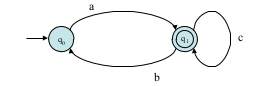
\includegraphics[scale=0.8]{img/aut.png}
\end{center}
in cui i nodi rappresentano degli stati e si ha uno stato inziale ($q_0$) e uno finale, denotato con un doppio cerchio, ($q_1$).\newline
Gli archi sono le transizioni tra due stati e nel nostro caso generano caratteri e nell'esempio ho soltanto stringhe che iniziano con $a$.\newline
In $q_1$ posso fermarmi e generare solo la stringa $a$ o produrre altri caratteri in numero variabile e le stringhe qui prodotte
saranno del tipo $ac^n(ba)^n$, con $n\geq 0$.\newline
Per decidere se una certa sequenza di simboli è riconosciuta dall’automa possiamo costruire il seguente predicato:
\begin{minted}{prolog}
/* definisco l'interprete */
accept([I | Is], S) :-
  delta(S, I, N),
  accept(Is, N).
accept([], Q) :- final(Q). /* è l'uscita, se ho una lista vuota
                               ho generato tutto */

/* richiesta di riconoscere un automa con stato iniziale S
    poi si usa l'accept con input che rappresenta la stringa
     considerando lo stato inziale S */
recognize(Input) :- initial(S), accept(Input, S).

initial(q0). % stato iniziale
final(q1). % stato finale

/* definisco le transizioni, con delta a tre argomenti */
delta(q0, a, q1).
delta(q1, b, q0).
delta(q1, c, q1).
\end{minted}
\begin{shaded}
\begin{lstlisting}[language=bash]
?- recognize([a, b, a, c, c, b, a]).
Yes

?- recognize([a, b, a, c, b]).
No
\end{lstlisting}
\end{shaded}
Per riuscire a comprendere come funziona l'interprete vediamo il suo funzionamento considerando la lista $[a,\,b,\,a,\,c,\,c,\,b,\,a]$,
in cui si hanno le seguenti sostituzioni: $I\backslash a$ e $S\backslash q0$.\newline
Avrò quindi:
\begin{minted}{prolog}
delta(q0, a, N).
accept([b, ...], N).
\end{minted}
Ora si effettuano le seguenti sostituzoni: $N\backslash q1$:
\begin{minted}{prolog}
accept([b, ...], q1). % è il nuovo goal
\end{minted}
unifico ancora con le sostituzioni $I2\backslash b$ e $Is\backslash [a,c,c,b,a]$:
\begin{minted}{prolog}
delta(q1, b, N2).
accept([a, c, c, b, a], N2).
\end{minted}
ad un certo punto arriveremo alla fine:
\begin{minted}{prolog}
accept([], q1).
\end{minted}
che unifica con la seconda clausola, sostituendo $q1\backslash Q$, arrivando a:
\begin{minted}{prolog}
final(q1).
\end{minted}
Dopo aver considerato come si definisce un interprete per automi, possiamo considerare degli interpreti più sofisticati
se accettiamo di rappresentare i programmi, usando una sintassi leggermente diversa:
\begin{minted}{prolog}
rule(append([], X, X)).
rule(append([X | Xs], Ys, [X | Zs]), [append(Xs, Ys, Zs)]).

solve(Goal) :- solve(Goal, []). /* lista goal e lista di appoggio
                                    dove mettere i goal restanti */

solve([], []). % clausola di uscita

solve([], [G | Goals]) :-
  solve(G, Goals).
solve([A | B], Goals) :-
  append(B, Goals, BGoals),
  solve(A, BGoals).
solve(A, Goals) :-
  rule(A),
  solve(Goals, []).
solve(A, Goals) :-
  rule(A, B),
  solve(B, Goals).
\end{minted}
Il programma \textit{solve} è un meta-interprete per i predicati rule che compongono il nostro sistema/programma Prolog.
Ovviamente fino ad ora abbiamo considerato di rappresentare dei sistemi perfetti, in cui si può inferire in maniera certa su dei fatti/regole
cosa che difficilmente nella realtà avviene, per cui soprattutto per definire degli interpreti per l'apprendimento automatico, per questo
aggiungiamo ad ogni predicato/fatto un argomento numerico, tra 0.0 e 1.0,
indicante la probabilità che il fatto/predicato risulti verificato.\newline
Ad esempio modifichiamo il precedente esempio per considerare l'incertezza:
\begin{minted}{prolog}
solve_cf(true, 1) :- !.
solve_cf((A, B), C) :-
  !,
  solve_cf(A, CA),
  solve_cf(B, CB),
  minimum(CA, CB, C).
solve_cf(A, 1) :-
  builtin(A),
  !,
  call(A).
solve_cf(A, C) :-
  rule_cf(A, B, CR),
  solve_cf(B, CB),
  C is CR * CB.
\end{minted}
Il programma $solve_cf$ è un meta-interprete per stabilire se un goal G è vero e quanto siamo certi che sia vero.
%Capitolo sulla programmazione logica in Prolog

\chapter{Lisp:Programmazione Funzionale}
Dopo aver affrontato ed analizzato il Prolog e il paradigma Logico, è arrivato
il momento di analizzare il paradigma ``matematico'' funzionale,
in cui la computazione risiede nel definire e applicare una serie di funzioni,
anche composte e soprattutto ricorsive.\newline
Nel paradigma funzionale risulta verificato il concetto matematico della \textbf{trasparenza refenziale},
funzione senza effetti collaterali che quando riceve lo stesso parametro in input,
restituisce sempre lo stesso valore, cosa non sempre verificata negli altri linguaggi.

L'uso della trasparenza referenziale ha il grande vantaggio di permettere al programmatore
di poter contare su un comportamento univoco delle funzioni, a priori non sempre prevedibili
e ciò aiuta molto nel processo di testing e debug, semplifica l'implementazione di algoritmi,
rende più facili la modifica e l'ottimizzazione dei programmi senza cambiarne radicalmente la struttura.

Nel paradigma funzionale vi sono oggetti di vario tipo e strutture di controllo, ma vengono raggruppati logicamente in modo diverso
da come invece accade nel paradigma imperativo, infatti risulta utile pensare in termini di:
\begin{itemize}
\item espressioni, il quale rappresenta i fondamenti del linguaggio come le funzioni semplici e primitive.
\item modi di combinare le espressioni per ottenerne di più complesse, tramite l'operazione di composizione
\item modi e metodi di costruzione ``astratte''  per poter far riferimento a gruppi di espressioni per “nome” e per trattarle come unità separate
\item operatori speciali (condizionali ed altri ancora, che verranno introdotti in seguito)
\end{itemize}

Noi affronteremo come esempio di linguaggio funzionale, il linguaggio Common Lisp, una dei principali dialetti, come anche lo Scheme, della famiglia
di linguaggi chiamati Lisp.\newline
Lo studio del Lisp, anche se in una delle sue incarnazioni, è importante dato che è il primo linguaggio di programmazione funzionale e
le sue versioni minimali ammettono:
\begin{itemize}
\item funzioni primitive su \textbf{liste}
\item un'operatore speciale \textbf{lambda} per creare funzioni
\item un'operatore codizionale \textbf{cond}
\item un piccolo insieme di predicati ed operatori speciali
\end{itemize}

Incominciamo a mostrare come valuta e computa le espressione il Common Lisp
e la prima cosa notata è che ogni ``espressione'' denota un valore.
\begin{minted}{Lisp}
prompt> 42
42

prompt> ”Sapete che cos’e` ’42’?”
”Sapete che cos’e` ’42’?”
\end{minted}
In Lisp sono presenti le operazioni aritmetiche principali(+ - * /), rappresentate in notazione prefissa,
il quale permettono di essere applicate a più argomenti ed evitano di generare ambiguità su quale operazione viene
applicata in caso di più operazioni, come si nota nei seguenti esempi:
\begin{minted}{Lisp}
  prompt> (+ 137 349)
  486

  prompt> (- 1000 334)
  666

  prompt> (+ 2.7 10)
  12.7

  prompt> (* 2 34)
  68

  prompt> (/ 10 5)
  2
\end{minted}
Queste espressioni, formate delimitanto una lista di espressioni all'interno di parentesi per mostrare l'applicazione di una funzione,
sono chiamate \emph{combinazioni} e il valore viene determinato applicando la procedura, specificata dall'operatore, agli argomenti,
i quali sono i valori degli operandi.
Le espressioni possono essere annidate, per cui per motivi di lettura si allineano gli argomenti di chiamata verticalmente, come nell'esempio:
\begin{minted}{Lisp}
prompt> (+ (* 3
              (+ (* 2 4)
                 (+ 3 2)))
           (+ (- 10 8)
              1))
42
\end{minted}
Notiamo come le funzioni aritmetiche elementari + e * in (Common) LISP rispettano i vincoli di “campo” algebrico:
\begin{minted}{Lisp}
prompt> (+)
0

prompt> (*)
1
\end{minted}
Un aspetto dei linguaggi di programmazione è quello di fornire dei nomi, per riferirsi agli oggetti computazionali,
ed ovviamente anche nel Common Lisp ciò avviene tramite l'istruzione $defparameter$, che si comporta nel seguente modo:
\begin{minted}{Lisp}
  (defparameter pi_greco 3.14)
  (defparameter size 2)
\end{minted}
Per valutare una espressione combinata, l'interprete Lisp esegue le seugenti operazioni:
\begin{enumerate}
\item viene valutata la sottoespressione, presente nella combinazione
\item viene applicata la procedura, rappresentata dalla sottoespressione left-most, agli argomenti
  rappresentati dai valori delle altre sottoespressioni.
\end{enumerate}
Ovviamente come si può notare la valutazione risulta ricorsiva e i componenti basilari, su cui si riesce ad effettuare correttamente la valutazione
sono i seguenti:
\begin{itemize}
\item il valore dei numeri sono ovviamente il numero stesso
\item il valore degli operatori built-in sono le istruzioni macchina che corrispondono a quell'operatore.
\item il valore degli altri nomi sono gli oggetti associati a quel nome nell'ambiente definito nel programma Lisp
\end{itemize}
Questo concetto per valutare le espressioni non si applica agli operatori speciali, come ad esempio defparameter.

In Lisp si hanno come dati e procedure predefinite il seguente elenco di elementi:
\begin{itemize}
\item numeri interi, numeri in virgola mobile (es. $3.5$ o $6.02E+21$), numeri razionali
      (es. $-3/42$) o numeri complessi ($\#C (0 1)$)
\item booleani $T$ e $NIL$
\item stringhe (es $"sono\,\,\, una \,\,\,stringa"$)
\item operatiori sui booleani $null,\,\,\,and,\,\,\, or,\,\,\,not$
\item funzioni sui numeri \textit{+ - / * mod sin cos sqrt tan atan plusp > <= zerop}
\end{itemize}
Per definire nuove funzioni, per fornire una forma di astrattezza e fornire il nome ad una serie di operazione,
in Lisp si usa il comando \mint{Lisp}|defun (nome (argomenti) (corpo funzione))|:
Ovviamente questa possibilità di definire nuove funzioni può essere combinato per creare
in maniera semplice nuove funzioni, come si può notare nel listato di esempio:
\begin{figure}
\caption{Esempi di definizioni di funzioni}
\begin{minted}{Lisp}
prompt> (defun square (x) (* x x))
square

prompt> (square 5)
25

prompt> (defun sum-of-square(x, y) (+ (square x) (square y)))
sum-of-square

prompt> (sum-of-square 3 4)
25
\end{minted}
\end{figure}
La definizione di nuove funzioni permette di creare un'astrazione e considerare la procedura come una ``black box'', in cui l'utilizzatore
della funzione può essere diverso da chi l'ha definita e la utilizza senza sapere i dettagli implementativi; ciò permette di poter cambiare
l'implementazione senza preoccuparsi di dover cambiare tutti i riferimenti ad essa e di avere i parametri a visibilità locale alla procedura.

Per valutare una espressione combinata dove un operatore indica una funzione composta, definita tramite \emph{defun}, l'interprete Lisp segue
lo stesso processo visto per valutare le funzioni/operazioni primitive, infatti l'interprete valutano gli elementi presenti nell'espressioni
e poi applicano la procedura agli argomenti, indicati dagli operandi nell'espressione.\newline
Per applicare una funzione composta agli argomenti si valuta il corpo della procedura in cui ogni parametro formale
viene sostituito dall'argomento corrispondente e per illustrare il processo vediamo come viene valutata la seguente espressione
!!!inserire esempio di applicazione di un'espressione

Il processo descritto e mostrato nel seguente esempio viene chiamato \textbf{substitution model} e lo scopo di questo processo è quello
di aiutare a pensare a come si applica alla procedura, ma non fornisce una descrizione fedele di come un interprete realmente lavora.

Inserire differenza tra applicazione e ordine normale


La potenza espressiva delle funzioni definite fino ad ora è limitata, dato che non abbiamo ancora la possibilità di effettuare delle scelte
e per risolvere introduciamo ora il costrutto speciale \textbf{cond}$(cond\,\,(p_1\,\,e_1),\,\,...\,\,(p_n\,\,e_n))$:
consiste in una coppia di espressioni, dove il primo elemento è sempre un predicato ``logico'', come si può notare nel listato di esempio.\newline
L'operatore cond verifica ogni coppia di espressioni e se il risultato è T ritorna il valore della seconda espressione altrimenti
passa alla coppia successiva fino a che se non ci sono più coppie valutabili restituisce NIL.\newline
In aggiunta ai predicati aritmetici, < > =, per effettuare dei confronti si possono utilizzare i predicati \textbf{and, or, not},
definiti come si nota nel seguente listato:
\begin{figure}
\begin{minted}{lisp}
prompt> (and (> 42 0) (< -42 0))
T

prompt> (not (> 42 0))
NIL

prompt> (and)
T

prompt> (or)
NIL
\end{minted}
\end{figure}

\begin{figure}
\begin{minted}{lisp}
(defun valore-assoluto (x)
   (cond ((> x 0) x)
         ((= x 0) 0)
         ((< x 0) (- x))))

prompt> (valore-assoluto 3)
3

prompt> (valore-assoluto -42)
42
\end{minted}
\end{figure}
Per rappresentare il valore assoluto, come si vede nel listato Y, si poteva utilizzare anche il predicato \mint{Lisp}
|(if <predicate> <conseguent> <alternative>)|, applicabile quando si hanno solo due casi da analizzare.\newline
Per valutare il predicato \emph{if} l'interprete inizia a valutare la parte <predicate> dell'espressione: in caso viene valutata con $T$
allora l'interprete valuta la parte <conseguent> e ritornaa il suo valore, altrimenti viene valutato la parte <alternative> e ritorna il suo valore.

\begin{figure}
\begin{minted}{lisp}
prompt> (define (abs x)
            (if (< x 0)
            (-x)
             x))
\end{minted}
\end{figure}
Nella definizione di una funzione è possibile che si abbia la necessità di usare delle funzioni ausiliarie, che può avvenire in maniera separata
oppure in maniera innestata, attraverso una definizione \emph{block structure}, il quale permette di isolare e non fornire ad altre funzioni
la procedura ausiliaria.\newline
La scelta tra i due modi dipende dal fatto se la procedura ausiliaria può essere usata all'in fuori della procedura oppure dipende sempre da essa:
nel primo caso si usa una definizione separata per poter usare da sola mentre nel secondo caso si utilizza una definizione innestata.

Vediamo una funzione ricoriva come il fattoriale:
\begin{minted}{lisp}
(defun fattoriale (n)
    (if (= n 0)
        1
        (* n (fattoriale (- n 1)))))
\end{minted}
Questa funzione calcola il fattoriale di un numero utilizzando una sequenza di valori intermedi che devono essere salvati sullo ``stack''
di attivazione di ogni chiamata ricorsiva e questa definizione matematica e ricorsiva del fattoriale richiede $\Theta(n)$ sia in tempo che spazio
per effettuare il fattoriale di un numero $n$ ma utilizzando una procedura iterativa, in cui ad ogni passo teniamo traccia del fattoriale
calcolato al passato, richiedendo uno spazio $\Theta(1)$ per effettuare la computazione, come si può nuotare nel seguente listato:
\begin{figure}
  \includeminted{Esempi/fattorialeRicorsivo.lisp}{Lisp}
\end{figure}
Con la procedura ausiliaria innestata  si ha la presenza sia di un ``ciclo in incognito'' non visibile all'esterno, che permette al compilatore di
ottimizzare, attraversola chiamata di una jump, e questa procedura ausiliaria viene detta \textbf{tail-recursive}.

Vediamo anche Fibonacci:
\begin{minted}{lisp}
(defun fib (n)
     (cond ((= n 0) 1)
           ((= n 1) 1)
           (T (+ (fib (- n 2)) (fib (- n 1))))
            ))
\end{minted}
In Lisp, come tutti i linguaggi funzionali essendo basati sul lambda-calcolo di Church,
si possono definire funzioni anonime, chiamate \textbf{funzioni lambda}, utili per
definire funzioni ausiliarie senza fornigli un nome ed un'esempio viene fornito dal listato:
\begin{figure}
\begin{minted}{Lisp}
       (lambda (x y) (* x y))
\end{minted}
\end{figure}
Le funzioni lambda forniscono una certa eleganza al codice e permettono di non associare
il nome a delle procedure ausiliarie, il cui utilizzo necessità di una procedura principale.
Usando l'operatore lambda possiamo costruire una serie di valori intermedi da
utilizzare per la computazione e questo utilizzo è talmente standard ed utilizzato
che il Lisp ha fornito l'operatore speciale \textbf{let}, per cui i seguenti listati
sono equivalenti:
LISTATO LAMBDA

LISTATO LET
IMPLEMENTAZIONE ITERATIVA DEL FIBONACCI
\section{Strutture Dati in Lisp}
Nei precedenti paragrafi abbiamo assunto e definito solo espressioni e funzioni che operano su numeri mentre i programmi sono solitamente
definiti su dati composti, al fine di rappresentare al meglio la realtà e di elevare il livello concettuale dei nostri programmi, permettendo
di avere una maggiore potenza espressiva del linguaggio.

Per vedere l'importanza e come definire un dato composto consideriamo ora la costruzione di una libreria per fare lavorare coi numeri razionali
ed innanzitutto assumiamo di aver a disposizione una funzione che costruisce una rappresentazione di un numero razionale:
\begin{minted}{lisp}
(make-rat n d) Þ <il razionale n/d>
\end{minted}
Assumiamo anche di avere due funzioni numer and denom che straggono rispettivamente il numeratore n ed il denominatore dalla
rappresentazione di un numero razionale <razionale n/d>:
\begin{minted}{lisp}
(defun somma-raz (r1 r2)
    (crea-razionale (+ (* (numer r1) (denom r2))
                       (* (numer r2) (denom r1)))
                    (* (denom r1) (denom r2))))
(defun molt-raz (r1 r2)
    (crea-razionale (* (numer r1) (numer r2))
                    (* (denom r1) (denom r2)))
(defun =-raz (r1 r2)
    (= (* (numer r1) (denom r2))
       (* (numer r2) (denom r1))))

...
\end{minted}
Questa definizione dei numeri razionali permettono di aumentare la modularità dei nostri programmi e di poter manipolare i numeri razionali,
senza conoscere come sono stati definiti.

Una delle strutture più importanti del Lisp è la \textbf{Cons-Cell}, ovvero una coppia di due elementi a cui si può accedere tramite
\textit{car e cdr}, il quale puntano al primo e secondo elemento, come si nota nel seguente listato di esempio:
\begin{figure}
\begin{minted}{Lisp}
prompt> (defparameter c (cons 40 2))
c

prompt> (car c)
40

prompt> (cdr c)
2
\end{minted}
\end{figure}
Una coppia è un oggetto a cui si può dare un nome e manipolare, come gli oggetti primitivi, e ciò permette di creare coppie annidate come si nota:
\begin{figure}
\begin{minted}{Lisp}
  prompt> (defparameter x (cons 1 2))
  x

  prompt> (defparameter y (cons 3 4))
  y

  prompt> (defparameter z (cons x y))
  z

  prompt> (car (car z))
  1

  prompt> (car (cdr z))
  3
\end{minted}
\end{figure}
La definizione delle coppie ci semplifica la libreria per i razionali, infatti definiamo un numero razionale tramite la seguente definizione:
con questo costrutto si semplifica la libreria per i razionali:
\begin{figure}
\begin{minted}{lisp}
(defun make-rat (n d)
                (cons n d))%rappresenta il costruttore

(defun numer (r) (car r))%rappresenta il selettore

(defun denom (r) (cdr r))%rappresenta il selettore

prompt> (denom (make-rat 42 7))
7
\end{minted}
\end{figure}

La funzione cons genera in memoria dei grafi di puntatori arbitrariamente complessi, rappresentati in una tradizionale notazione
detta \textit{box-and-pointer}:
\begin{figure}
\centering
\includegraphics[scale=0.7]{img/cons.png}
\end{figure}
Posso inserire anche T e NIL (rappresentato da una sbarra):
\begin{figure}
\includegraphics[scale=0.7]{img/cons2.png}
\end{figure}
Vediamo qualche esempio:
\begin{figure}
\begin{minted}{Lisp}
prompt> (cons NIL T)
(NIL . T) ; Notazione “dotted-pair”
          ; (“coppia-puntata”). Gli spazi
          ; sono significativi.

prompt> (cons 4 2)
(4 . 2)
\end{minted}
\end{figure}
Un altra utile struttura dati, definibile attraverso l'uso delle pairs, è la lista, sequenza ordinata di oggetti, rappresentabile in varie maniera
ma la più immediata consiste una serie di pair, dove la car di ogni pair rappresenta un elemento mentre la cdr è un riferimento
al prossimo elemento della lista che può essere NIL.\newline
La definizione della sequenza $(1, 2, 3, 4)$ in Common Lisp viene definito nel seguente listato:
\begin{figure}
\begin{minted}{Lisp}
  (defparameter L (cons 1 (cons 2 (cons 3 (cons 4)))))
\end{minted}
\end{figure}

\begin{center}
  \includegraphics[scale=0.7]{img/cons3.png}
\end{center}
Una lista Lisp corrispondente a questa configurazione di cons-cells viene rappresentata tipograficamente come \textit{((T) 42)} che è equivalente
a \textit{((T . NIL) . (42 . NIL))}.\newline
Quindi una cons-cell con NIL come secondo elemento (ovvero come cdr) viene stampata senza il punto ed il NIL:
\begin{minted}{Lisp}
prompt> (cons 42 nil)
(42)

prompt> (cons ”foo bar” nil)
(”foo bar”)
\end{minted}

\begin{figure}
\begin{minted}{lisp}
  (defparameter L (list 1 2 3 4))

  prompt> (car (cdr (cdr L)))
  3
\end{minted}
\end{figure}
L'implementazione delle operazioni standard definite sulle liste si può notare
nel listato di esempio:
INSERIRE LISTATO SULLE liste

La definizione di funzioni ricorsive sulle liste può essere semplice, in caso si
effettuano le chiamate ricorsive solo sulla coda, oppure doppia in caso si lavora
sia sulla testa che sulla coda della lista.%Inserire esempi

Per estrarre un elemento di una lista si utilizza la funzione standard \textbf{nth}
ed inoltre la funzione \textbf{cdr} ritorna il "resto" di una lista, come fatto
anche dalla funzione \textbf{rest}.\newline
Per ottenere il primo elemento di una lista si può usare la funzione \textbf{car}
oppure la funzione standard \textbf{first}.

Se si volesse definire in Lisp una lista del tipo $(A B C D)$, per quello che
abbiamo visto fino ad ora, non sarebbe possibile dato che l'interprete Lisp con l'espressione
                     cercherebbe di valutare la funzione list, applicata ai simboli $A, B, C, D$
ma ciò causa un errore, non essendo i simboli associati a qualche valore nell'ambiente,
come si nota nel listato di seguito:
\begin{figure}
\begin{minted}{Lisp}
prompt> (list A B C D)
ERRORE A NON HA NESSUN VALORE ASSOCIATO

prompt> (list 'A 'B 'C 'D)
(A B C D)
\end{minted}
\end{figure}
Per poter gestire i dati simbolici, come ad esempio la lista $(A B C D)$ oppure
$(+ quaranta 2)$ senza procedere alla valutazione delle espressioni, si ha la funzione
$quote <e>$, rappresentabile anche con $'<e>$;
la funzione quote sui numeri e stringhe è inutile dato che la loro valutazione è
identica alla rappresentazione data mentre serve per rappresentare i dati simbolici,
come le espressioni composte e/o rappresentazione di una sequenza di elementi,
come si nota nel listato ADD:
\begin{figure}
\begin{minted}
prompt> '42
42

prompt> '"la gatta ha fretta"
la gatta ha fretta

prompt> (list 'A 'B)
(A B)

prompt> '(defun media (x y) (/ (+ x y) 2.0))
(DEFUN MEDIA (X Y) (/ (+ X Y) 2.0))
\end{minted}
\end{figure}
FARE LA VALUTAZIONE DELLA FUNZIONE EVAL

In Lisp per controllare se due oggetti sono uguali vengono forniti una molteplicità
di funzioni built-in ma le principali sono le seguenti:
\begin{description}
  \item [eql:] viene usato per controllare l'uguagianza di simboli, numeri interi e stringhe
  \item [equal:] è in grado anche di controllare se due liste sono uguali e questa funzione
         non fa altro che applcare eql ricorsivamente a tutti gli atomi della lista.
\end{description}

\section{Funzioni di ordine superiore}
Dopo aver analizzato come si definiscono le liste, le funzioni e come essere in grado
in modo simbolico i dati, grazie all'operatore speciale quote, possiamo considerare
gli aspetti e  della programmazione funzionale.

Incominciamo delle funzioni di ordine superiore, il quale sono delle funzioni che
prendono uno o più funzioni come argomenti e possono ritornare anche una funzione.

Questa possibilità rappresenta il cuore e l'essenza della programmazione funzionale
e le principali funzioni standard di ordine superiore sono le seguenti:
\begin{description}
  \item [mapcar:] rappresenta l'astrazione di applicare la funzione f a tutti gli
         elementi della lista L e ritorna una lista di valori.
         Può essere definita, anche se è già built-in, nel seguente modo:
         \begin{minted}{Lisp}
              (defun mapcar (funzione lista)
                     (if (null lista)
                          null
                          (cons (funcall funzione (car lista))
                                 (mapcar funzione (cdr lista)))))
         \end{minted}
  \item [compose:] rappresenta la composizione di funzioni, ossia date due funzioni
                   $f$ e $g$, di un solo parametro, come argomenti viene ritornata
                   una nuova funzione corrispondente a $f(g(x))$.\newline
                   Può essere definita nel seguente modo:
                   \begin{minted}{Lisp}
                   (defun compose (f g)
                          (lambda (x)
                                  (funcall f (funcall g x))))
                   \end{minted}
  \item [filter:] rimuove gli elementi della lista che non soddisfano il predicato
                 e può essere definito nella seguente maniera:
                 \begin{minted}{Lisp}
                 (defun filter (predicato lista)
                        (cond ((null lista) nil)
                              ((funcall predicato (car lista))
                               (cons (car lista)
                                     (filter predicato (cdr lista)))
                              (T (filter predicato (cdr lista))))))
                 \end{minted}
  \item [accumula:] applica una funzione ad un elemento di una lista e il risultato
                    dell'applicazione ricorsiva di accumula al resto della lista;
                    la definizione di questa funzione potrebbe essere la seguente:
                    \begin{minted}{Lisp}
                    (defun accumula (f iniziale lista)
                           (if (null lista)
                               iniziale
                               (funcall f (car lista)
                                        (accumula f iniziale (cdr lista)))))
                    \end{minted}
\end{description}
In common Lisp alcuni simboli hanno un interpretazione particolare, per esempio
i simboli iniziati con : vengono detti \textbf{keywords} ed hanno come valore se stesso,
come si può notare nel listato XXTTT.
\begin{esempio}
  \begin{minted}{Lisp}
  cl-prompt> :foo
  :foo

  cl-prompt> :forty-two
  :forty-two
\end{minted}
\end{esempio}
Le keywords vengono utilizzate in maniera estesa in Common Lisp e servono essenzialmente
per definire delle funzioni con una sintassi di chiamata più utile ed interessante,
ma prima di parlarne vediamo ora le sequenze variabili di argomenti, chiamate \textbf{lambda list}.

In Common Lisp è possibile definire delle funzioni che prendono un numero variabile di argomenti,
come si può notare nel listato CCCCCC, utile per permettere l'applicazione della funzione
a più argomenti possibili.\newline
È disponibile anche definire delle funzioni con dei parametri opzionali, infatti basta
usare la sintassi utilizzata nel listato ffsdafdfd, che possono essere inizializzati
con un valore di default.

In Common Lisp si possono definire delle funzioni che utilizzano i loro parametri
associandoli alle keyword e ciò è molto comune infatti molte funzioni standard
hanno questo comportamento, come si nota nel listato di esempio XXXXXX.

Ovviamente si possono definire delle funzioni che accettano parametri keywords, ovvero
ogni parametro passato in questa maniera diventa una keyword da poter utilizzare
al momento della chiamata della funzione, come si nota nel listato XXXXXXXX.

Questi parametri opzionali, a chiave e variabili devono essere sempre dichiarati
dopo i parametri obbligatori e il loro utilizzo è molto pervasivo in Common Lisp,
anche se noi non abbiamo visto le regole più sofisticate per il loro utilizzo.


\section{Input ed Output}
Dopo aver analizzato il paradigma funzionale e la sua essenza, ci concentriamo ora
sulla gestione dell'input ed output in Common Lisp: le due funzioni principali per
questo scopo sono \textbf{read} e \textbf{print}.

La funzione READ legge un intero oggetto Lisp, riconoscendone la sintassi, come
si può notare nel listato fsffsfsfsdsdfa, mentre la funzione PRINT stampa un oggetto
Lisp rispettandone la sintassi e il valore ritornato è il valore dell'oggetto la
cui rappresentazione è appena stata stampata, come si nota nel listato DDFGGGG.

Ovviamente queste funzioni sono molto grezze per cui è bene avere a disposizione
dei metodi per poter stampare in maniera più agevole, per questa maniera il Common Lisp
mette a disposizione la funzione molto complessa FORMAT(simile alla fprintf in C/C++).







Il linguaggio Lisp mette a disposizione una linea di comando interattiva, il quale
effettua il ciclo \textbf{READ-EVAL-PRINT}:
\begin{enumerate}
  \item READ: legge l'espressione inserita e viene rappresentata internamente in
        strutture dati appropriate(numeri, caratteri, simboli, stringhe ed ecc...)
  \item EVAL: viene valutata l'espressione inserita e dato che programmi e sexp's
        in Lisp sono equivalenti possiamo dare le seguenti regole di valutazione:
        \begin{itemize}
          \item Se una sexp's è un atomo ritorna il suo valore se è una stringa o un numero,
                in caso sia un simbolo viene estratto il suo valore corrente e viene ritornato
                invece se non esiste un valore associato al simbolo viene segnalato un errore.
          \item Se una sexp's è una cons-cell $(O A_1 A_2 \dots A_n)$ allora si procede nel seguente modo:
                \begin{itemize}
                  \item se $O$ è un operatore speciale la lista $(O A_1 \dots A_n)$
                        viene valutata in maniera speciale
                  \item se $O$ è un simbolo che denota una funzione nell'ambiente corrente
                        allora la funzione viene applicata alla lista $(VA_1 VA_2 \dots VA_n)$
                        indicanti i valori delle valutazioni degli argomenti della funzione.
                  \item Se $O$ è una espressione lambda la si applica agli argomenti
                  \item Altrimenti si segnala errore
                \end{itemize}
        \end{itemize}
  \item PRINT: viene stampato il risultato dell'espressione a video
\end{enumerate}
Le funzioni \textbf{apply} e \textbf{eval}, necessarie per valutare le espressioni,
possono essere scritte direttamente in Lisp, anche se sono già implementate in maniera standard,
in quanto in Lisp i dati e i programmi sono la stessa cosa.

Grazie a questo aspetto è possibile scrivere un interprete Lisp nel linguaggio stesso,
chiamato \textbf{interprete meta-circolare}, e cominciamo ora definendo la funzione valuta(eval è standard)
a partire dalle regole di valutazione definite.

La funzione valuta prende una sexp's e un ambiente env e ritorna una sexp's e procede nel seguente modo:
\begin{enumerate}
  \item 
\end{enumerate}



     (Parte della funzione EVAL E READ EVAL PRINT LOOP)
Lisp languages are often used with an interactive command line, which may be combined with an integrated development environment (IDE). The user types in expressions at the command line, or directs the IDE to transmit them to the Lisp system. Lisp reads the entered expressions, evaluates them, and prints the result. For this reason, the Lisp command line is called a read–eval–print loop (REPL).

The basic operation of the REPL is as follows. This is a simplistic description which omits many elements of a real Lisp, such as quoting and macros.

The read function accepts textual S-expressions as input, and parses them into an internal data structure. For instance, if you type the text (+ 1 2) at the prompt, read translates this into a linked list with three elements: the symbol +, the number 1, and the number 2. It so happens that this list is also a valid piece of Lisp code; that is, it can be evaluated. This is because the car of the list names a function—the addition operation.

Note that a foo will be read as a single symbol. 123 will be read as the number one hundred and twenty-three. "123" will be read as the string "123".

The eval function evaluates the data, returning zero or more other Lisp data as a result. Evaluation does not have to mean interpretation; some Lisp systems compile every expression to native machine code. It is simple, however, to describe evaluation as interpretation: To evaluate a list whose car names a function, eval first evaluates each of the arguments given in its cdr, then applies the function to the arguments. In this case, the function is addition, and applying it to the argument list (1 2) yields the answer 3. This is the result of the evaluation.

The symbol foo evaluates to the value of the symbol foo. Data like the string "123" evaluates to the same string. The list (quote (1 2 3)) evaluates to the list (1 2 3).

It is the job of the print function to represent output to the user. For a simple result such as 3 this is trivial. An expression which evaluated to a piece of list structure would require that print traverse the list and print it out as an S-expression.

To implement a Lisp REPL, it is necessary only to implement these three functions and an infinite-loop function. (Naturally, the implementation of eval will be complex, since it must also implement all special operators like if or lambda.) This done, a basic REPL is one line of code: (loop (print (eval (read)))).

The Lisp REPL typically also provides input editing, an input history, error handling and an interface to the debugger.

Lisp is usually evaluated eagerly. In Common Lisp, arguments are evaluated in applicative order ('leftmost innermost'), while in Scheme order of arguments is undefined, leaving room for optimization by a compiler.

\end{document}
